\documentclass[a4paper, 12pt]{article}

% ------------------------------------------------------------------------------
%
%        VGTU FMF MSK BAKALAURINIO DARBO ŠABLONAS
%        Pagrindinių paketų rinkinys, viršelis ir bazinė dokumento struktūra
%
%        Autorius: Tomas Rekašius      tomas.rekasius@vgtu.lt
%
%         Sukurta: 2015-05-28
%       Pataisyta: 2017-05-14
%         Versija: 1.1
%

% ------------------------------------------------------------------------------
%  PREAMBULĖ
% ------------------------------------------------------------------------------

\usepackage[utf8]{inputenc}            % naudojama, kai .tex failas UTF-8 koduotės
\usepackage[L7x]{fontenc}              % nurodoma lietuviško teksto koduotė Latin-7
\usepackage[lithuanian]{babel}         % nurodoma, kad dokumentas yra lietuviškas

\usepackage{lmodern}                   % dokumente naudojamas šriftas Latin Modern
\usepackage{microtype}                 % optimizuojami atstumai tarp raidžių žodyje
\usepackage{indentfirst}               % atitraukiama pirmoji naujo skyriaus eilutė
\usepackage{icomma}                    % po kablelio skaičiaus viduryje nebus tarpo
\usepackage{amsmath, amssymb, amsthm, bbold}  % matematiniai simboliai ir konstrukcijos
\usepackage{graphicx}                  % grafinių failų įterpimas ir kiti nustatymai
\usepackage{booktabs}                  % reikalingas tvarkingoms lentelėms sudaryti
\usepackage{caption}                   % paveiksliukų ir lentelių užrašų formavimas
\usepackage{geometry}                  % paraščių ir kitų lapo parametrų nustatymai
\usepackage{hyperref}                  % interaktyvioms nuorodoms dokumente sukurti
\usepackage{array}
\usepackage[ruled,vlined,onelanguage]{algorithm2e}
\usepackage{algorithmic}

\geometry{      left = 2.5cm,          % paketo geometry parametrų nustatymai
               right = 2.0cm, 
                 top = 2.0cm, 
              bottom = 2.0cm
}

\captionsetup{format = hang,           % paketo caption parametrų nustatymai
           labelfont = bf,
           tablename = lentelė,
          figurename = pav,  
            labelsep = period
}

\hypersetup{ unicode = true,           % paketo hyperref parametrų nustatymai
         linktocpage = false, 
          colorlinks = true, 
           linkcolor = red,
           citecolor = blue,
            pdftitle = {VGTU FMF MSK bakalaurinio darbo šablonas},
           pdfauthor = {Paulius Janėnas}
}


% PAPILDOMI PAKETAI IR NUSTATYMAI ----------------------------------------------

\usepackage{titlesec}                  % leidžia keisti skyriaus pavadinimo stilių
\titlelabel{\thetitle.\quad}           % dedamas taškas po skyriaus numeriu tekste

\let\tocnumdot\numberline              % uždeda tašką po skyriaus numeriu turinyje
\def\numberline#1{\tocnumdot{#1.}}     


\linespread{1.3}                       % nustatomas 1,5 dydžio tarpas tarp eilučių

\graphicspath{{figures/}}              % nustatome kelią iki paveiksliukų katalogo 
\SetKw{KwBy}{by}
\SetKwInput{KwResult}{Rezultatas}%
\SetKwInput{KwData}{Duomenis}%
\SetKwInput{KwIn}{Algoritmas}%
\setcounter{algocf}{0}

\newcommand\mycommfont[1]{\footnotesize\ttfamily\textcolor{blue}{#1}}
\SetCommentSty{mycommfont}



% ------------------------------------------------------------------------------
%  DOKUMENTO PRADŽIA
% ------------------------------------------------------------------------------
\begin{document}


% ------------------------------------------------------------------ VIRŠELIS --

\begin{titlepage}
\setcounter{page}{-2}
\centering
%

\includegraphics[scale = 0.6]{vgtu_herbas}\\[0.5\baselineskip]
%
{\Large\scshape Vilniaus Gedimino Technikos Universitetas}\\[0.2\baselineskip]
{\large\scshape Fundamentinių mokslų fakultetas}\\[0.2\baselineskip]
{\large\scshape Matematinės statistikos katedra}\\[0.2\baselineskip]
%
\vspace{\fill}
%
{\Large Justina Marcinkėnaitė}\\[3.0\baselineskip]

\MakeUppercase{\Large\bfseries Statistinė inkstų veiklos sutrikimo analizė}\\[0.3\baselineskip]
{\Large The statistical analysis of renal dysfunction}\\[1.0\baselineskip]

{\Large Baigiamasis bakalauro darbas}

\vspace{\fill}

Taikomosios statistikos ir ekonometrijos studijų programa, valstybinis kodas 612G31001

Statistikos studijų kryptis


\vspace{\fill}
%
Vilnius, \the\year
\end{titlepage}


% ----------------------------------------------------------------- TITULINIS --

\begin{titlepage}
\setcounter{page}{-1}
\centering
%
{\Large\scshape Vilniaus Gedimino Technikos Universitetas}\\[0.2\baselineskip]
{\large\scshape Fundamentinių mokslų fakultetas}\\[0.2\baselineskip]
{\large\scshape Matematinės statistikos katedra}\\[0.2\baselineskip]
%
\vspace{\fill}
%
\begin{flushright}
\parbox{6cm}{%
TVIRTINU\\Katedros vedėjas
\bigskip
\begin{center}
\hrule\medskip
{\footnotesize (Parašas)}\\[\baselineskip]
\hrule\medskip
{\footnotesize (Vardas, pavardė)}\\[\baselineskip]
\hrule\medskip
{\footnotesize (Data)}
\end{center}
}
\end{flushright}
%
\vspace{\fill}
%
{\Large Justina Marcinkėnaitė}\\[3.0\baselineskip]

\MakeUppercase{\Large\bfseries Statistinė inkstų veiklos sutrikimo analizė}\\[0.3\baselineskip]
{\Large The statistical analysis of renal dysfunction}\\[1.0\baselineskip]

{\Large Baigiamasis bakalauro darbas}

\vspace{\fill}

Taikomosios statistikos ir ekonometrijos studijų programa, valstybinis kodas 612G31001

Statistikos studijų kryptis

\vspace{\fill}
%
\begin{minipage}[t]{0.15\textwidth}
\bfseries Vadovas
\end{minipage}
%
\hspace{\fill}
%
\begin{minipage}[t]{0.4\textwidth}
\centering\hrule\medskip\scriptsize (Pedagoginis vardas, vardas, pavardė)
\end{minipage}
%
\hspace{\fill}
%
\begin{minipage}[t]{0.2\textwidth}
\centering\hrule\medskip\scriptsize (Parašas)
\end{minipage}
%
\hspace{\fill}
%
\begin{minipage}[t]{0.15\textwidth}
\centering\hrule\medskip\scriptsize (Data)
\end{minipage}


\vspace{\fill}
%
Vilnius, \the\year
\end{titlepage}


% ------------------------------------------------------------------- TURINYS --
\tableofcontents
\newpage

\cleardoublepage
\phantomsection
\addcontentsline{toc}{section}{\listfigurename}
\listoffigures
\newpage

\cleardoublepage
\phantomsection
\addcontentsline{toc}{section}{\listtablename}
\listoftables
\newpage



% -------------------------------------------------------------------- ĮVADAS --
\section*{Įvadas}
\phantomsection
\addcontentsline{toc}{section}{Įvadas}
%
Šių laikų žaidimų industrijoje sukurti žaidimo agentą, kuris realistiškai reaguoja į aplinką, yra sudėtinga užduotis reikalaujanti daug laiko bei pastangų. Taip pat neretai prie laiko kaštų prisideda ir tai, kad prieš kuriant žaidimo agentą tam reikia tinkamai paruošti aplinką – sukurti pagalbinius įrankius leidžiančius supaprastinti programavimo procesą. Tačiau net įdedant pastangas programuojant agentus, rezultatai yra dažnai prasti, jie nėra pakankamai protingi, žaidėjui nėra didžiulio iššūkio juos įveikti. Tai priveda prie didžiausio žaidėjų nepasitenkinimo – agentu sukčiavimo. Norint agentus padaryti protingesniais jiems suteikiama žaidimo informacija, kuri yra neprieinama įprastiems žaidėjams. 

Per pastarajį dešimtmetį įvykus neuroninių tinklų proveržiui buvo dedama daug vilčių, kad jie sugebės sukurti protingesnius žaidimo agentus. Tačiau neuroniai tinklai tėra funkcijos aproksimacijos metodas ir sunkiausia šio išukio dalis greitai atsiskleidė - kaip sukurti funkciją, kuri padėtų agentams tobulėti, tapti protingesniams? Šis klausimas buvo nagrinėtas per pastaruosius 70 metų, įtraukiant tokias mokslo šakas kaip dinaminis programavimas, markovo modeliai, neuromokslai. Atradimai minėtose šakose privedė prie skatinamojo mokslo gimimo, kuomet 1987 metais šio mokslo pradininkai Sutton, R. bei Barto, A. moksliniame straipsnyje \cite{TDSutton} pirmieji sukūrė optimizavimo funkciją, pavadinta "Temporal difference" (toliau TD), padedančia agentams mokytis iš praeities rezultatų, siekiant pasirinkti tokius ateities veiksmus, kurie pagerintų ateities rezultatą. Funkcijos principas remiasi skatinimo metodais, kaip siunčiant paskatinimo impulsus agentui, jei jis atliko teisinga veiksmą, bei nubaudžiamas jei atliko neteisingą veiksmą. Tokiu principu agentas sukuria pozityvias bei negatyvias asociacijas su galimais veiksmais, kuriuos jis gali atlikti. Šį principą puikiai iliustruoja pavlovo šunų eksperimentas. Sekančius dešimtmečius sekė šios funkcijos gerinimas, optimizavimas, bandymas išspręsti didelės dimensijos problemą - kuo didesnė dimensija, tuo ilgiau užtrunka skaičiavimai. Ši problema buvo išspresta pasitelkiant neuroninius tinklus, kurie aproksimuodavo TD funkciją. Šio metodo kulminacija įvyko 2016 metais, kuomet Google AlphaGo sugebėjo įveikti stalo žaidimą Go, kurio nesugebėjo įveikti nei viena komanda prieš tai dirbusi prie pirmųjų algoritmų, įveikusių šachmatų čempionus. Šiuo metu skaitinamieji metodai aprėpia daugybe sričių: automobilių autonominis vairavimas, logistikos grandžių optimizavimas, robotikos judėjimo problemos ir dar daugybe kitų sričių. 

Šiame darbe bus išanalizuojamas skatinamasis mokymasis bei įgyvendintas vienas iš šio mokslo metodų - TD3. Teorinėje dalyje bus analizuojama šio metodo veikimo principai. Tai atlikus praktinėje dalyje šis metodas bus pritaikytas išspręsti roboto voro fizinio judėjimo aplinkoje problemą.



%
\paragraph{Darbo aktualumas.} Dirbtiniui intelektui sugebėjus įveikti šachmatų čempionus buvo manoma, kad žmonių dominavimas tradiciniuose stalo žaidimuose pasibaigė. Tačiau programuotojų ambicijos išblėso, kuomet min-max paremti šachmatų algoritmai nesugebėjo įveikti kiniečių tradicinio stalo žaidimo – Go. To pagrindinė priežastis – neapskaičiuojamai didelė žaidimo būsenų erdvė. Kompiuteriai užtrukdavo per ilgai planuoti ėjimus ir jam neužtekdavo atminties išanalizuoti visus galimus ėjimus. Todėl iki šiol šis stalo žaidimas buvo neįveikiamas iki kol Google korporacija išleido skatinamojo mokymosi paremto algoritmo, kuris 2016 metais sugebėjo įveikti šių laikų geriausią Go žaidėją. Nuo to laiko skatinamųjų mokymosi metodų aktualumas vis labiau plito įtraukiant sritis kaip autonominiai automobiliai, robotika, finansai bei vis naujai populiarėjanti sritis – žaidimų industrija. 
%
\paragraph{Darbo tikslas} Pritaikyti TD3 skaitinamojo mokymosi modelį, kuris apmokytų simuliuojamą vorą vaikščioti 3D aplinkoje.
%
\paragraph{Uždaviniai.} Maecenas eget erat in sapien mattis porttitor:
%
\begin{enumerate}
  \addtolength{\itemsep}{-0.5\baselineskip} 
  \item Išanalizuoti gilių neuroninių tinklų struktūrą.
  \item Įgyvendinti Python bei Unity duomenų sinchronizaciją.
  \item Išanalizuoti skatinamojo mokymosi modelio principus.
  \item Išanalizuoti Belmano, Q-mokymosi, TD funkcijas.
  \item Sukurti unity voro aplinką bei agentą, kuris bus apmokomas vaikščioti.
  \item Įgyvendinti TD3 mokymosi modelį bei apmokyti vorą vaikščioti sukurtoje aplinkoje.
\end{enumerate}


%
%
\newpage



% ------------------------------------------------------------------- SKYRIUS --
\section{Teorinė dalis}
%

Skatinamojo mokymo metodai remiasi neuroninių tinklų aproksimacijom. Todėl šioje darbo dalyje nagrinėsiu giliųjų neuroninių tinklų veikimo principus. Tai atlikęs toliau nagrinėsiu skatinamojo mokymosi metodus bei kaip neuroniniai tinklai padeda juos įgyvendinti. Pagrindinis nagrinėjamas skatinamojo mokymosi modelis bus TD3. Tai yra modelis kuris padeda agentui tolydžioje aplinkoje pasirinkti veiksmus, kurie suteike dydžiausią apdovanojimą. Galiausiai bus nagrinėjama aplinka, kurioje šis mokymo metodas bus įgyvendintas.

%
\subsection{Neuroninių tinklų klasifikatorių tipai}
%

%
\subsubsection{Neuroninio tinklo struktūra}
%

Neuroninių tinklų sandarą galimą žiūrėti kaip į daugybės logistinių funkcijų veikimą. Kitaip tariant vieną neuroną galima traktuoti kaip logistinę funkciją, kuri išsiskaido į dvi dalis: tiesinę bei aktyvacinę. Tiesinėje dalyje suskaičiuojame tiesinę lygtį ir ją įvedame į aktyvacijos funkciją, kuri logistinėje regresijoje yra sigmoido funkcija. Tai yra identiška logistinei regresija, kurios išvedimus buvau pateikęs praeitoje ataskaitoje. Aktyvacinės funkcijos gali būti skirtingos, nebūtinai sigmoido. Pagrindinė skirtingų aktyvacinių funkcijų priežastis yra spartesnė svorių konvergacija į optimalią reikšmę. Dažnai naudojama Relu aktyvacinė funkcija, kuri neturi sigmoido nykstančio gradiento problemos. Ši problema pasireiškia kuomet sigmoido funkcijos reikšmė yra labai didelė arba maža, tuomet gradientas tampa beveik nulinis ir mokymosi procesas sustoja. 
Pats neuroninis tinklas susideda iš logistinių funkcijų (jei naudojame ne sigmoid aktyvacinę funkciją tai jau nebėra logistinė funkcija) sluoksnių, kurie prasideda įvesties sluoksnių, viduryje paslėptuoju sluoksniu ir galiausiai išvesties sluoksniu. Visi klasifikatoriai turi vieną bendrą panašumą – įvesties bei paslėptuosius sluoksnius. Tačiau priklausomai nuo to ar atsakas yra klasifikacinis ar regresinis, kinta išvesties sluoksnis. Kuriant python aplinkoje neuroninius tinklus buvo pasitelkta vektorizacija. Visus įvestis, svorius, išvestis išsireiškus matriciniu pavidalu gaunamas ryškus neuroninių tinklų paspartėjimas. Neuroninio tinklo bendra naudota struktūra yra pateikta \ref{neuronu diagrama} pavekslėlyje.

\begin{figure}[h]
\centering
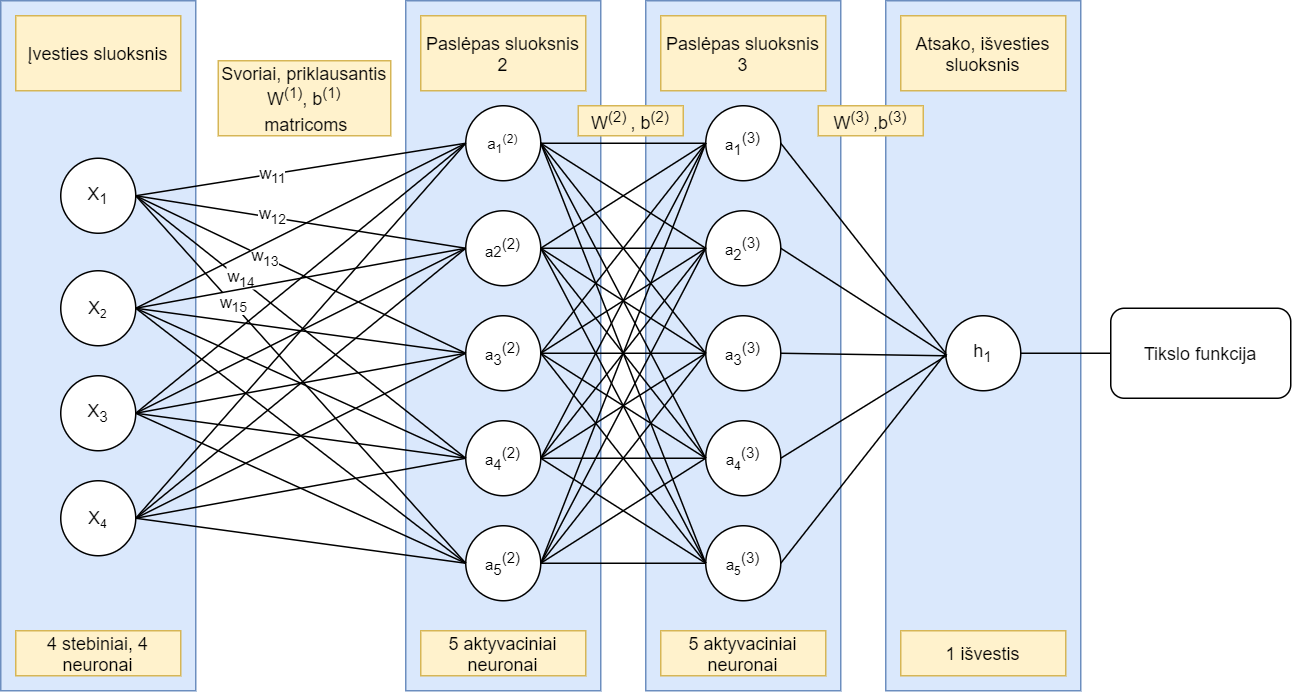
\includegraphics[width=1\textwidth]{neuronu diagrama}
\caption{Gilaus neuroninio tinklo bendra struktūra}
\label{neuronu diagrama}
\end{figure}

Vieno sluoksnio įvesties transformacijos vektorizaciją yra taip skaičiuojama:

$$
Z^{l}=W^{{l}^T} * A^{l-1}+b^{l}
$$

Žymėjimas: $A^l$ yra $l$ sluoksnio įvestis (matrica, kuri susideda iš $a^l$ elementų) gauta po aktyvacinės funkcijos (jei $l$ yra lygus įvesties sluoksniui, tai $A^l$ tampa duomenų įvesties vektorius $X$), o $W^T$ yra to sluoksnio svoriai.
Šios transformacijos matricos eilutės yra skirtingų neuronų tiesinės transformacijos reikšmės, o stulpeliai žymi skirtingus mokymosi duomenis. Šią transformaciją įkėlus į aktyvacijos funkciją gauname galutinę perceptrono reikšmę.
Norint, kad neuroninis tinklas būtų tikslus, mes turime optimizuoti svorius. Tam pasitelkiame gradientinį nuolydį. Gradientinis nuolydis padeda surasti svorius su kuriais tikslo funkcija įgyja mažiausią paklaidą. Tikslo funkcija sudaro tolygų paviršių, kurio skiringos ašys yra svorių reikšmės bei viena iš jų yra tikslo funkcijos rezultatas. Pateiktame \ref{gradientinis nuolydis} pavekslėlyje apatines ašis $x$ bei $y$ galima traktuoti kaip svorius, o viršutinę ašį kaip tikslo funkcijos paklaidą. 

\begin{figure}[h]
\centering
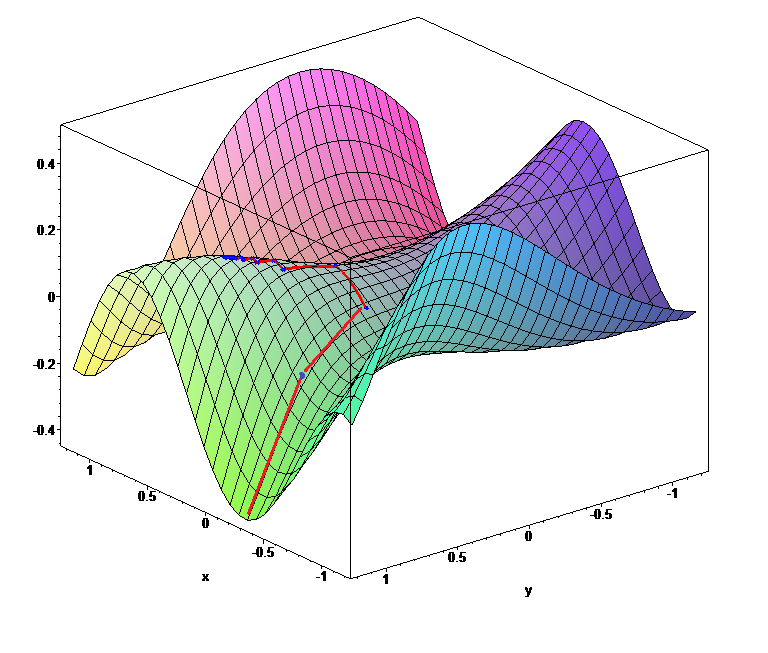
\includegraphics[width=0.7\textwidth]{gradientinis nuolydis}
\caption{Gradientinio nuolydžio pavyzdys}
\label{gradientinis nuolydis}
\end{figure}

Judandami svorius priešingą gradiento puse, mes judame ties tokiais svoriais, kurie mažiną tikslo funkcijos paklaidą. Šią trajektoriją atspindi 
\ref{gradientinis nuolydis} pavekslėlyje esanti raudona tiesė, kuri kiekvienos iteracijos metu (mėlyni taškai) po truputi slenka žemyn, optimizuoja svorius.

Vėlgi gradientinio nuolydžio vektorizacija yra tokia pati tiek įvesties, tiek paslėptuose sluoksniuose, bet priklausomai nuo analizuojamos problemos - skirtinga išvesties sluoksnyje. Gradiento vektorizacija:

\begin{equation}
\label{eqn:backpropdz}
d Z^{l}=W^{l+1^{T}} d Z^{l+1} * g^{l}\left(Z^{l}\right)
\end{equation}

Žymėjimas: $g^l(Z^l)$ yra dabartinio sluoksnio aktyvacinės funkcijos išvestinė. Ji yra sudauginama su visais matricos nariais. Gavus perceptronų išvestines $dZ^l$ toliau galime gauti svorių gradientus:


\begin{equation}
\label{eqn:backprop}
\begin{gathered}
d W^{l}=\frac{1}{m} d Z^{l} A^{(l-1)^{T}} \\
d b^{l}=\frac{1}{m}\left(d Z^{l} \text { matricos stulpeliu susumavimas }\right)
\end{gathered}
\end{equation}



Žymėjimas: stulpelių skaičius arba mokymosi duomenų kiekis yra žymimas $m$. Toliau bus aptariamos priekinio, atgalinė propogacija bei tikslo funkcijos, kurios sudaromos atitinkamai pagal turima klasifikacijos problemą.

%
\subsubsection{Neuroninio tinklo priekinė propogacija}
%

Įgyvendinti gilaus neuroninio tinklo struktūra pasirinktoje programavimo kalboje nėra sunku, kuomet pastebimas visiems sluoksniams bendras pasikartojantis skaičiavimo bruožas. Skaičiuojant priekinę propogaciją (judame neuriniu tinklu iš kairės į dešinė) į neuroninį tinklą galima žiurėti kaip į atskirus blokus susidedančius iš įvesties bei išvesties, kaip tai matosi \ref{forwardProp} paveikslėlyje.
\clearpage
\begin{figure}[h]
\centering
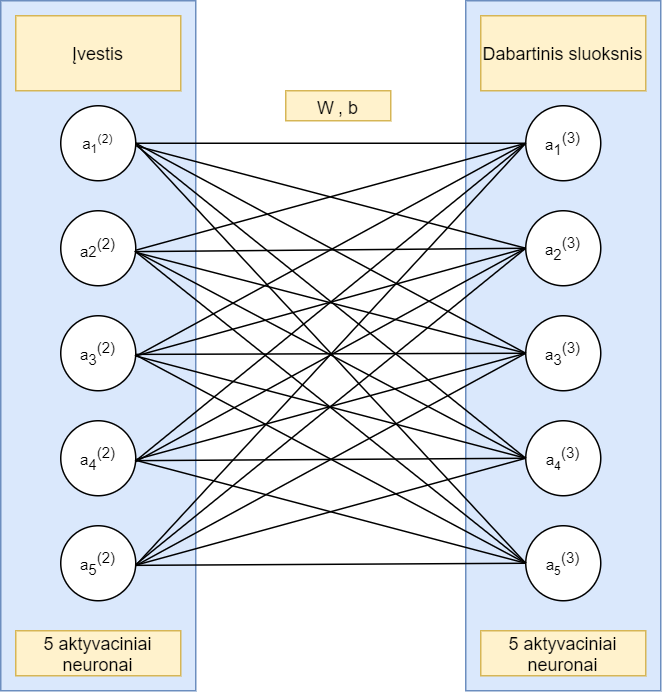
\includegraphics[width=0.6\textwidth]{ForwardProp}
\caption{Priekinės propogacijos vieno neuroninio sluoksnio apskaičiavimo grafas}
\label{forwardProp}
\end{figure}

Tokia formą išskaidžius neuroninį tinklą, jį tampa labai paprasta apskaičiuoti, tereikia iteruoti kiekvienu sluoksniu iš kairės į dešinę. Kiekvienos iteracijos metu praeitą sluoksnį traktuojame kaip įvesties sluoksnį ir naudojantis \ref{eqn:backprop} formulėmis apskaičiuojame dabartinio sluoksnio aktyvacinius neuronus. Šios operacijos metu svarbu išsaugoti tarpinius skaičiavimus, kaip tiesinės funkcijos bei aktyvacinę funkcijos apskaičiavimo rezultatą. Jos bus reikalingos apskaičiuoti gradientinį nuolydį, kaip tai matosi \ref{eqn:backpropdz} bei \ref{eqn:backprop} formulėse. Paskutinės iteracijos metu, atlikus aktyvacinės funkcijos apskaičiavima, lieka tik apskaičiuoti tikslo funkcijos rezultatą. 
Šį struktūra pasižymi formulių universalumu, jos tinka neuroniniams tinklams, kurie yra negilieji bei gilieji, kitaip tariant - nepriklauso nuo sluoksnių kieko. Atlikus priekinę propgaciją ir suskaičiavus tikslo funkcijos klaidą, galime pradėti ją mažintį, judėdami priešinga gradiento linkme. Tai atlieka sekanti potemė - atgalinė propogacija.
	

%
\subsubsection{Neuroninio tinklo atgalinė propogacija}
%

Atgalinės propogacijos struktūra yra vos ne identiška priekiniai propogacijai. Pagrindiniai skirtumai yra sukeistos vietos apskaičiuojamo sluoksnio bei įvesties sluoksnio. Tačiau kaip ir priekinės propogacijos atveju, mes atliekame panašias įteracijas, tik šį kart pradedam nuo tiklso funkcijos ir judame link pirmo sluoksnio, iš kairės į dešinę. Atliekant šias svorių atnaujinimo operacijas, kaip tai matosi \ref{eqn:backpropdz} bei \ref{eqn:backprop} formulėse, pasitelkiame priekinės propogacijos metu išsaugotais duomenimis. 

\begin{figure}[h]
\centering
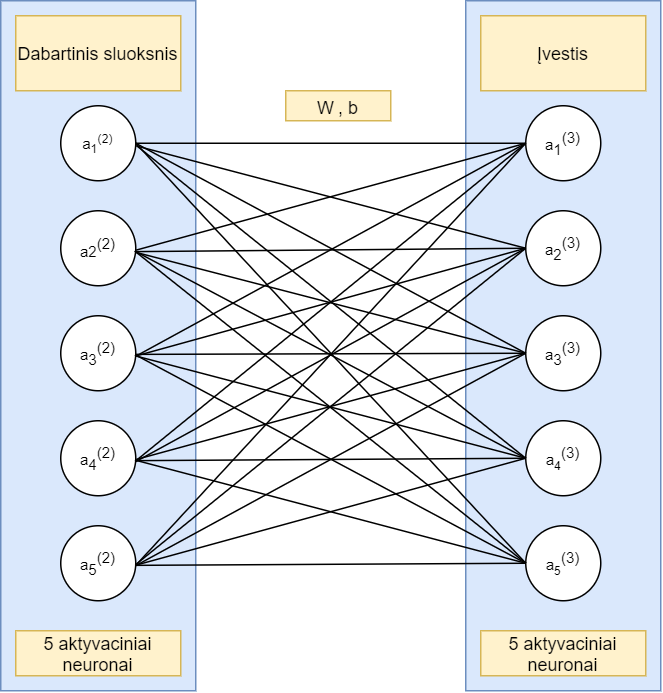
\includegraphics[width=0.6\textwidth]{BackProp neuronais}
\caption{Atgalinės propogacijos vieno neuroninio sluoksnio apskaičiavimo grafas}
\label{BackProp neuronais}
\end{figure}

%
\subsubsection{Binarinis klasifikatorius}
%

Tai klasifikatorius, kuris vos ne identiškas logistinei regresijai. Klasifikuoja binarinius atsakus. Išvesties sluoksnis turi tik vieną neuroną bei jo reikšmės transformacija sutampa su logistinės regresijos tikslo funkcija:

\begin{equation}
\log (L)=\ell=\sum_{i=1}^{n}\left[y_{i} \log \left(p_{i}\right)+\left(1-y_{i}\right) \log \left(1-p_{i}\right)\right]
\end{equation}

Šios funkcijos neurono gradientas yra susiprastiną į šią formą:

\begin{equation}
d Z^{l}=A^{l}-Y,
\end{equation}

kur $l$ yra paskutinis sluoksnis, $Y$ yra tikroji atsako reikšmės, o $A^l$ yra neuroninio tinklo gauti atsakai. Turint $dZ^l$ galima gauti svorių gradientus bei neuronų gradientus, kaip tai buvo parodyta prieš tai. Turint svorių gradientus atnaujiname svorius:

\begin{equation}
W^{l}=W^{l}-\alpha dW^{l}
\end{equation}

kur $\alpha$ nurodo gradientinio žingsnio dydį.

%
\subsubsection{Daugiau nei viena klasė}
%

Klasifikuojant daugiau nei vieną klasę yra naudojamas entropijos tikslo funkcija. Tikslo funkcijos forma:

\begin{equation}
L(y, \hat{y})=-\sum_{i=1}^{N} y_i * \log (\hat{y_i}),
\end{equation}
kur $y$ yra tikroji reikšmė, o $\hat{y}$ yra aproksimuota.


Kuomet paskutinio sluoksnio aktyvacinė funkcija yra „soft-max“, šios funkcijos gradientas labai gražiai susiprastina ir paskutinio sluoksnio gradientas atrodo ši taip:

\begin{equation}
d Z^{l} = (Y- \hat{Y})
\end{equation}

kur $l$ yra paskutinio sluoksnio indeksas, o dydžiosios $Y$ yra vektorizacija daugybės stebinių į vieną matricą.

Iš šio gradiento galime seniau aptartais metodais gauti $W$ bei $b$ gradiento reikšmes. Galima naudoti ir didžiausių kvadratų metoda, tačiau gradientinis nuolydis konverguotų lėčiau.
Taip pat pagrindinis skirtumas tarp binarinio klasifikatoriaus yra aktyvacinė funkcija. Šį kart tai nėra sigmoido funkcija, o „soft-max“ normalizacija. Jos metu kiekvieno neurono reikšmės apskaičiuojamos naudojantis eksponento funkcija $e^z$, visos reikšmės padalinamos iš šių reikšmių sumos ir gautas rezultatas perduodamos į tikslo funkciją. Taigi šis metodas yra dažnai naudojamas klasifikuoti reikšmes, kurios turi daugiau nei vieną klasę.

%
\subsubsection{Tiesinės regresijos atsakas}
%

Jei atsakas yra regresinis, tuomet tikslo funkcija tampa didžiausių kvadratų optimizacijos tikslo funkcija ir paskutinis neuronas neturi aktyvacijos funkcijos. Tikslo funkcijos dydžiausių kvadratų sumos vidurkio formulė:

\begin{equation}
MSE=\frac{1}{N} \sum_{i=1}^{N}\left(y_i-\hat{y_i}\right)^{2}
\end{equation}
kur $y$ yra tikroji reikšmė, o $\hat{y}$ yra aproksimuota.

Neuroniniai tinklai su regresinę tikslo funkciją yra puikus agentų apmokymo pavyzdys, įrodantis kad priklausomai nuo užduoties, nebūtina imtis sudėtingų skatinamojo mokymosi metodų, norint sukurti protingą agentą. Su šiuo metodu buvo optimizuojamas stalo teniso žaidimas, kuriame atsakas buvo stalo teniso raketės pozicijos optimali padėtis atmušti atskriejanti kamuoliuką, kaip tai matosi \ref{pingpong} paveikslėlyje. Tai buvo paprastas gilus neuroninis tinklas su dveis paslėptais sluoksniais po 12 neuronų. Buvo pasitelktas stochastinis gradientinis nuolydis, kuomet kiekvieno žaidimo kadro metu buvo nusiunčiami neuroniniam tinklui dabartinės raketės padėtis bei kamuoliuko trajektorija. Šiam uždaviniui neuroninio tinklo nereikia, pakaktu paprasto algoritmo ar tiesinės regresijos, tačiau tai gerai iliustruoja jo veikimo principus. Pradžioje raketės juda padrikai, bet bėgant laikui, vykstant gradientiniui apsimokymui, rakečių judėjimas vis tikslėja.

\begin{figure}[h]
\centering
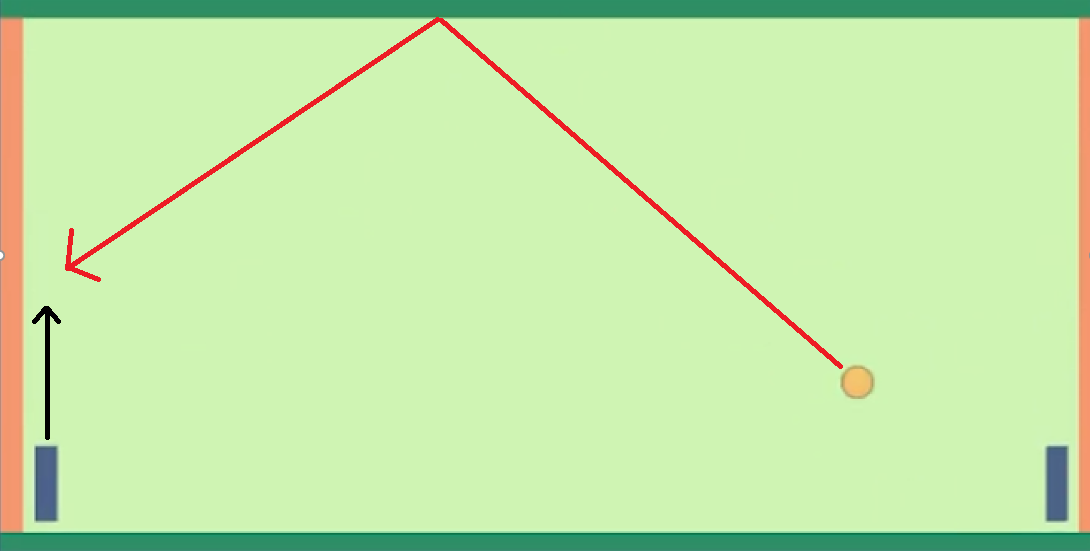
\includegraphics[width=1\textwidth]{pingpong}
\caption{Sukonstruota stalo teniso simuliacija}
\label{pingpong}
\end{figure}

\ref{pingpong} Paveikslėlyje raudona trajektoriją yra neuroninio tinklo įvestis, apskaičiuojanti kamuoliuoko galutinę padėtį. Juoda trajektorija yra neuroninio tinklo išvestis, raketės greičio vektorius, simbolizuojantis pozicija, kurioje raketė turi atsirasti

%
\subsubsection{Tiesinė regresija su daugybe atsako kintamųjų}
%

Identiška tiesinės regresijos funkcijai, tačiau šiuo atveju paskutinis sluoksnis turi daugiau nei vieną neuroną. Tuomet tikslo funkcija atrodo šitaip:

$$
L=\frac{1}{m * 2} * \sum\left(Z^{l}-Y\right)^{2}
$$

Vektorizacija identiška tiesinės regresijos atveju, tik atsako kintamasis Y turi ne vieną eilutę, o daugiau. Eilutės žymi pasirinkto sluoksnio neuronų reikšmes.
Su šiuo metodu buvo optimizuotas automobilio kontroleris, kurio tikslas buvo apvažiuoti trasą. Įvestis buvo normalizuota automobilio sensorių informacija, kurie pateikinėdavo trasos barjero atstumą. Išvestis buvo automobilio stabdymo ir greičio pedalo stiprumai bei vairo pozicija. Apmokius neuroninį tinklą rezultatai buvo tragiški, automobilis važiuodavo tik tiesiai. Tačiau pritaikius Adamo gradientinį nuolydį ir taip sumažinus modelio klaidą, buvo pasiekti tenkinami rezultatai. Automobilis sugebėdavo apvažiuoti trasą. 

%
\subsection{Neuroninių tinklų reguliarizacija}
%

Neuroninių tinklų reguliarizacija reikalinga norint išvengti modelio prisitaikymo prie mokymosi duomenų. Ji padeda pagerinti testavimo duomenų tikslumą. Toliau nagrinėsiu metodus, kurie tai padeda pasiekti.

%
\subsubsection{L1 bei L2 reguliarizacija}
%

Didžiuliai svoriai retai gerai generalizuoja modelį, jie numuša testavimo imties tikslumą. Todėl svarbu neleisti svoriams tapti milžiniškais. L1 bei L2 reguliarizacija tai padeda pasiekti. Prie tikslo funkcijos lygties mes pridedame Lagrandžo svorių apribojimus L2 atveju:

$$
J(W, b, X, y)=\frac{1}{m} \sum L(y, \hat{y})+\frac{\lambda}{2 * m} \sum\left\|w^{l}\right\|^{2},
$$
kur $\lambda$ yra lagrandžo daugiklis ir taip pat hiperparametras.

Matome, kad prie pagrindinės tikslo funkcijos prisideda papildoma bauda, kuo didesni svoriai, tuo didesnė bauda. L1 atveju mes vietoj ilgio kvadrato, naudojame absoliutinę reikšmę. L2 skiriasi nuo L1 tuo, kad L2 padeda nunulinti tuos svorius, kurie turi mažai įtakos gradientiniam nuolydžiui, kaip tai matosi \ref{regularization} paveikslėlyje. Tačiau abiejais atvejais mes nepasieksime optimalios reikšmės ir išmainysime „variance“ į „bias”, taip pasiekdami tikslesnį testavimo duomenų klasifikavimą, jei modelis yra per daug prisitaikęs prie mokymo duomenų.
Gradientą šiai funkcijai lengva surasti, kadangi matome, kad $J$ funkcija išsiskaido į dvi dalis. Telieka surasti išvestines L2 formai, kas yra labai paprasta.

\begin{figure}[h]
\centering
\includegraphics[width=1\textwidth]{regularization}
\caption{Reguliarizacija - po kaire L1, po dešine L2}
\label{regularization}
\end{figure}

%
\subsubsection{Atvirkštinis išmetimas}
%
Šio metodo esmė, išjunginėti kiekvieno sluoksnio neuronus su tam tikra tikimybe. Juos išjungus, kiti neuronai turės perimti jų darbą ir papildomai apsimokyti. Tai padeda išvengti atveju, kuomet vienas neuronas persimoko. Tačiau išmetimo atveju vidutiniškai neuronų išvestis sumažėja išmetimo tikimybės procentu. Todėl atvirkštiniu išmetimu, mes po išmetimo operacijos kiekvieną neurono $Z$ reikšmę padaliname iš išmetimo tikimybės taip padidindami neurono išvestį ir gražindami to sluoksnio tikėtiną reikšmę.



%
\subsubsection{Duomenų augmentacija}
%

Šis metodas taikomas, kuomet neturime pakankamai duomenų. Jei duomenys susideda iš nuotraukų, tuomet augmentacijos metu mes galime nuotraukas apsukti, priartinti, karpyti ir panašius metodus taikyti, norint padidinti mokymosi duomenų imti.

%
\subsubsection{Įvesties normalizacija}
%

Gradientinio nuolydžio konvergacijos greitis priklauso nuo paviršiaus išsidėstimo. Paviršius gali būti labai susipaudęs bei banguotas, kas neleidžia atlikti didžiulių gradientinių žingsnių. Tokiais atvejais dideli žingsniai, gali šokinėti aplink optimalią reikšmę bei tokiu budu niekados nekonverguoti. Taip pat svoriai nėra proporcingai panašus, vieni turi žymiai didesnę įtaka nuolydžiui, kiti mažesne. Tokiu atveju paimti dideli gradiento žingsniai gali vėlgi nekonverguoti. Tačiau normalizavus įvesties duomenis, paviršius išsilygina bei yra lengviau optimizuoti. Normalizavimas paremtas paprasčiausiu statistiniu $Z$ normalizavimu. Jis atliekamas, kuomet įvesties duomenis pasižymi skirtingais duomenų intervalais – vienos įvesties intervalas [0,1], kitos [0,1000].

%
\subsection{Neuroninių tinklų parametrų inicializacija}
%


%
\subsubsection{Gradiento sprogimas bei nykimas, aktyvacinių funkcijų parametrų priskirimas}
%

„Forward propogation“ neuroninio tinklo žingsnyje, kuomet skaičiuojame išvestį galime pastebėti tokį neuroninio tinklo bruožą

$$
\hat{y}=W^{l} * W^{l-1} * W^{l-2} * \ldots * X
$$

Matome, kad jei $W^l$ parametrai priskiriami su didelėm reikšmėm, turint daugybe sluoksnių mūsų tiek neurono tiek svorių reikšmės ekponentiškai išauks. Tuo tarpu jei parametro reikšmės $W^l$ priskiriamos su mažesnėms nei vieneto reikšmėm, svoriai greitai tampa nuliais. Norint to išvengti visų neurono sluoksnio aktyvacijų reikšmių vidurkis turi būti lygus nuliui bei variacija visuose sluoksniuose išlikti vienoda. Šių tikslų padeda pasiekti svorių priskirimo metodai. Dažniausiai svoriai yra paimami iš $\mathcal{N}(0,1)\ast0.001$. Šie svoriai nėra blogi jei turime tik pora sluoksnių tačiau didėjant sluoksniams, kaip matėme prieš tai, neuronų reikšmės taps nuliais. Todėl priklausomai nuo sluoksnio aktyvacijos naudojame specifinius metodus priskiriant svorius. Kad šie metodai veiktų, įvestis privalo būti normalizuojama $Z$-norm principu. 

\begin{enumerate}
  \addtolength{\itemsep}{-0.5\baselineskip} 
  \item 	Jei aktyvacijos funkcija yra tanh, svoriai imami iš $\mathcal{N}(0,\frac{1}{n^{l-1}})$, kur n yra neuronų skaičius sluoksnyje, šiuo atveju tai būtų praeito sluoksnio neuronų skaičius.
  \item 	Jei aktyvacijos funkcija yra Relu, svoriai imami iš $\mathcal{N}(0,1)\ast\frac{2}{\sqrt n}$.
  \item 	Jei aktyvacijos funkcija yra sigmoidas, svoriai imami iš $\frac{\mathcal{N}(n^{l-1},n^l)}{\sqrt n}$.
\end{enumerate}

%
\subsection{Mokymosi greičio didinimas }
%
Jei turime labai daug duomenų, matricų operacijos užima daug laiko. Todėl naudojame tolimesnius metodus, kurie paspartina mokymosį procesą.

%
\subsubsection{Mažos mokymosi imties metodas}
%

Metodo principas labai paprastas – iš visos duomenų imties paimame dalį skirstinio ir su šia gauta maža mokymosi imtimi apmokome modelį. Kiekviena tokia dalis negražins optimalaus gradiento vektoriaus, tačiau kadangi duomenis yra iš to pačio pasiskirstimo mes vis tiek judėsime į optimalias svorių reikšmes ir galiausiai konverguosime į optimalius svorius.

%
\subsubsection{Stochastinis nuolydis}
%

Beveik toks pats kaip praeitas metodas, tik dar ekstremalesnis atvejis – gradientas gaunamas iš vieno imties elemento, stulpelio. Vektorizacija šiuo atveju praranda visą savo greitį, taip pat gradiento vaikščiojimas neatrodo tolygus, juda vos ne į visas puses. Tačiau bendra gradientų krypties tendencija juda link tikslo funkcijos klaidos mažinimo. To priežastis yra išlieka tokia pati, kaip praeito metodo: kadangi duomuo yra iš to pačio pasiskirstimo mes vis tiek judėsime į optimalias svorių reikšmes. Šis metodas yra nuolatos taikomas skaitinamuosiuose mokymosi metoduose.

%
\subsection{Gradientinio nuolydžio optimizavimas}
%

Norint pasiekti greitesni svorių konvergavimą yra sukurta skirtingų gradientinio nuolydžio metodų, kurie netik pagreitina konvergaciją bet ir padeda kovoti su didelėmis gradiento problemomis – keliavimas plokščiu paviršiu bei lokalus minimumai.

%
\subsubsection{Momentinis gradientinis nuolydis bei eksponentinškai pasvertų svorių vidurkis}
%

Pagrindinis šio optimizavimo principas remiasi momentiniu nuolydžiu, kuomet gradientas įgyja pagreiti ties dažniausiai pasikartojančiu vektoriumi. Primena įsibėgėjusi automobilį. Šis įsibegėjimas padeda išvengti lokalių minimumu, kaip tai matosi \ref{momentinisGreitis} paveikslėlyje. Jame pavaizduoti skirtingi gradientinio mokymosi algoritmai, kurie pradeda tame pačiame taške bei kurių dauguma sustoja mokytis ties lokaliu minimumu. Tačiau momentinio mokymusi paremti gradientinio nuolydžio metodai praskrieja lokalųjį minimumą, kuris tik trumpam sumažina gradiento greitį. Taigi momentinio greičio intuicija labai paprasta: jei gauname nauja gradiento reikšmę, kuri nurodo judėti priešinga linke, ji yra atsveriama gradieno įsibėgėjimo greičiu ir gradientas tik truputi suletėja. Šio gradiento formulė primena eksponentiškai pasvertų svorių vidurkio formulę ir išsireiškia tokiu pavidalu:

\begin{equation}
V d w=\beta_{1} * V d w+\left(1-\beta_{1}\right) * d w
\end{equation}

Kur $\beta_1$ yra parametras nuo 0 iki 1, dažniausiai būnantis 0.9. Kaip matome naujausi gradientai prie galutinės gradiento reikšmės prisidės tik $(1-\beta_1)$ dydžiu, kas suteikia momentinio greičio pavidalą. Šis pasvertų vidurkių principas yra plačiai naudojamas skatinamuosiuose mokymosi metoduose ir jį galima pastebėti visuose pagrindinėse formulėse. Skatinamuosiuose mokymosi metoduose šios formulės principą galima traktuoti kaip gradientinį nuolydį - po truputi konverguojame ties optimaliomis reikšmėmis.

\begin{figure}[h]
\centering
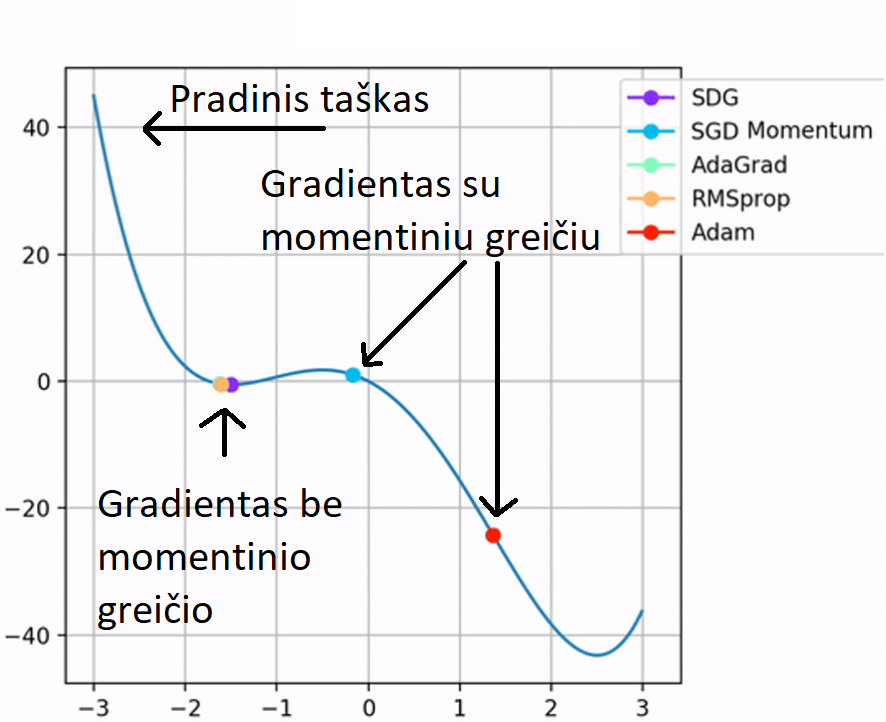
\includegraphics[width=.7\textwidth]{momentinisGreitis}
\caption{Gradientinė optimizacija su ir be momentinio greičio. SGD momentinis bei Adam konverguoja į globalų minimumą, like konvergavo į lokalų minimumą}
\label{momentinisGreitis}
\end{figure}


%
\subsubsection{Normalizuotas gradientinis nuolydis}
%

Niekur nenaudojamas gradientinio nuolydžio metodas, kurio metu gradiento dydis normalizuojamas. To pasekoje net ir plokštumoje greitis nėra nulinis. Tačiau mokymosi procesas yra labai lėtas, nes gradiento smarkus nuolydis yra normalizuojamas.

%
\subsubsection{RMSProp}
%

Tai gradientinio nuolydžio metodas, kurio tikslas pagreitinti gradientą, kuomet judame lygia plokštuma. Tačiau kaip matome iš \ref{momentinisGreitis} RMSProp kenčia nuo momentinio greičio neturėjimo ir sustoja ties lokaliu minimumu. RMSProp forma labai panaši į momentinio gradiento:

\begin{equation}
S d w=\beta_{2} * S d w+\left(1-\beta_{2}\right) *(d w)^{2}
\end{equation}

Ir svorių atnaujinimo formulė:

\begin{equation}
W=W-\alpha \frac{d w}{\sqrt{S d w}}
\end{equation}

Empiriškai galime pastebėti, kad didžiulios gradiento reikšmės sumažės, tačiau mažos padidės. Todėl šis metodas padeda išspręsti lėtą judėjimą lygumomis. Rekomenduojamas $\beta_2$ dydis yra 0.99.

%
\subsubsection{Adam}
%

Šis metodas yra vienas populiariausių gradientinio nuolydžio metodų. Jo tikslas sumažinti dvi problemas - lokalius minimumus bei judėjima plokštuma. Tai pasiekiame sukombinuojant momentininį greitį bei RMSProp:

\begin{equation}
W=W-\alpha \frac{V d w}{\sqrt{S d w}}
\end{equation}

$Vdw$ suteikia momentinį greitį kiekvienam svoriui. Bet jei momentinis greitis yra didelis $Sdw$ jį sumažiną. Tačiau jei gradientas užstringa lygumoje, $Sdw$ padeda atstrigti.
Šį metodą pritaikiau minėtame automobilio kontrolerio pavyzdyje. Jis padėjo pasiekti trygubai mažesnį klaidos dydį ir taip pagerino automobilio kontrolerį.


%
\subsection{Skatinamasis mokymasis}
%

Skatinamojo mokymosi metodai yra mašinio mokymosi metodai, kurie apdovanoja pageidaujamus veiksmus bei baudžia nepageidautinus veiksmus. Naujuosiuose skatinamuosiuose modeliuose apdovanojimo bei baudos dydis tėra vienintelė informacija, kurią modelis težino. Jei tiesinėje regresijoje mes nuolatos turėdavome tikrąsias reikšmes, ties kuriomis bandėme pritaikyti modelį, šiuo atveju tokia informacija yra nepasiekiama. Todėl mūsų modelis turi nuolatos tyrinėti aplinką, kaupti naujas patirtis. Šiuos duomenis gauname iš aplinkoje esančio roboto ar agento, kuris duotoje aplinkoje stengesi atlikti optimalius veiksmus ir pagal juos susidaryti geriausių siūlomų veiksmų modelį. 

Šią veiksmų eigą apibendrina bendrasis skatinamųjų modelių grafikas, pateiktas \ref{RLmodel} paveikslėlyje. Jis iliustruoja praktinės dalies pagrindinės užduoties įgyvendinimą, voro aštuonių galunių judinima, kuriomis bandoma kuo arčiau priartinti vorą ties žaliu kubeliu. 
\clearpage

\begin{figure}[h]
\centering
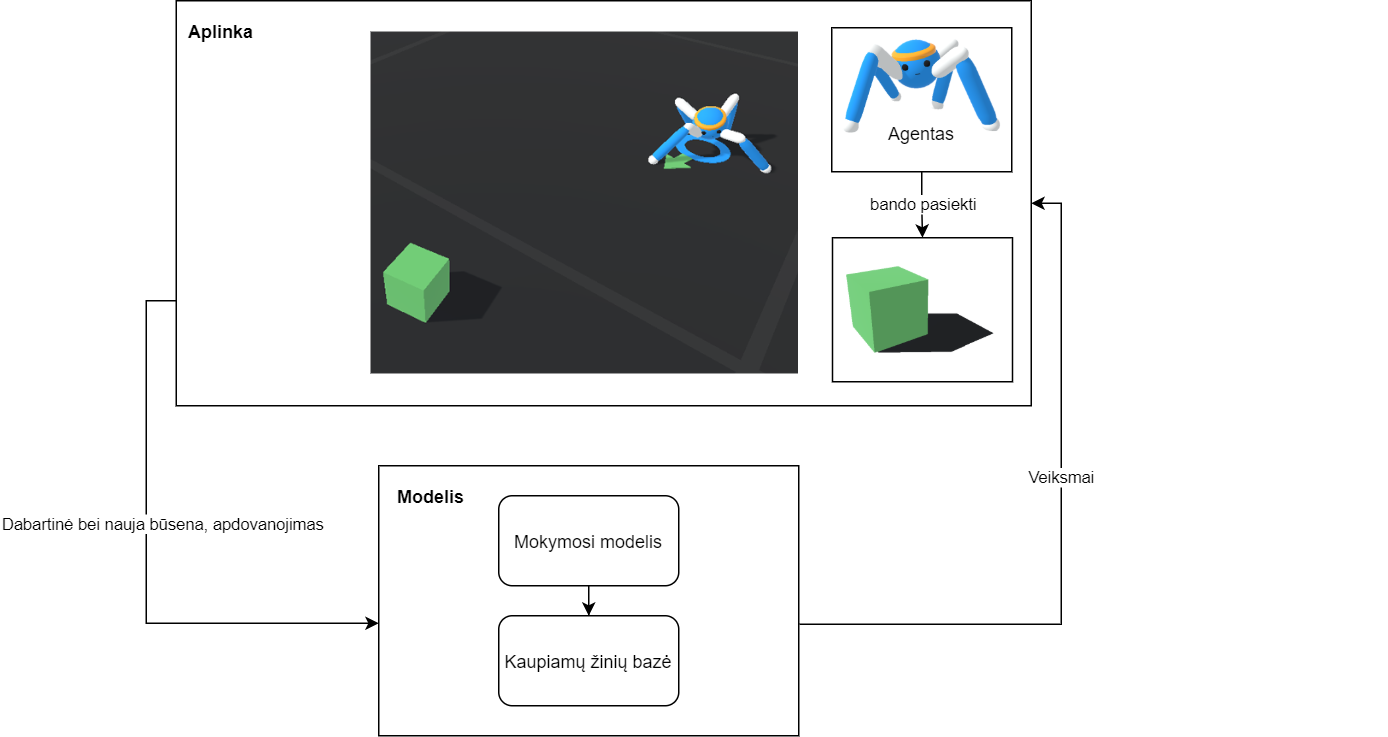
\includegraphics[width=1.3\textwidth]{RLmodel}
\caption{Bendras skatinamojo mokslo modelis}
\label{RLmodel}
\end{figure}



Šio modelio veikimo principai išsiskaido į šias dalis:
\begin{enumerate}
  \addtolength{\itemsep}{-0.5\baselineskip} 
  \item Aplinka. Aplinkoje egzistuoja mūsų agentas, kuris priiminėje modelio sugeneruotus veiksmus. Pateiktame pavyzdyje tai būtų voro galūnių judėjimo trajektorijos. Atlikes duotus veiksmus, voras įgauną naujas būsenas, pasistumį į naują poziciją. Nauja įgyta būsena bei prieš tai buvusi, nusiunčiama modeliui. Taip pat modeliui nusiunčiame apdovanojimo dydį. Jis apskaičiuojamas naudojantis naujai sugeneruotos būsenos naudingumu. Naudojantis voro pavyzdžiu tai atitiktų voro greičio vektorio laipsnio sutapimu su norimos krypties vektoriumi, kaip tai matosi \ref{voroGreicioVektoriai} pavekslėlyje. Šiuo atveju apdovanojimas būtų nulinis, nes vektorių trajektorijos visai nesutampa. Atlikus veiksmą bei apskaičiavus jo naudingumą, tokiu budu gaunamas ryšys tarp veiksmo, kuris sugeneruoja naują būseną, bei įgyto apdovanojimo, naujoje būsenoje. Šis ryšys tarp veiksmo bei gauto rezultato yra neseniai atgimusio skatinamojo moklso pamatas, kuriuo moderniausi algoritmai ne per seniausiai pradėjo vadovautis, atradus apdovanojimų taisyklių gradientą bei pradėjus taikyti neuroninius tinklus. 
  \item Agentas. Agento sluoksnis susideda iš mokymosi modelio bei žinių bazės, kurioje kaupiami gauti aplinkos rezultatai, susidedantis iš vektorių su šiomis reikšmėmis - praeita būsena, atliktas veiksmas, nauja būsena ir apdovanojimas. Mokymosi modelis naudojasi sukauptų žinių baze gerinti savo modelio rezultatus. Modelio tikslas yra pateikti tokias veiksmų sekas, kurios suteiktų dydžiausią įmanoma apdovanojimą. Voro pavyzdžiu tai būtų sėkmingas žalio kubelio pasiekimas. Modelio apmokymui yra sukurta daugybe įvairių metodų ir šiame darbe bus nagrinėjamas vienas iš jų - TD3
\end{enumerate}

\begin{figure}[h]
\centering

\includegraphics[width=1\textwidth]{voroGreicioVektoriai}
\caption{Apdovanojimo pavyzdys, pagal voro greičio (raudona rodyklė) bei norimo judėjimo (žalia rodyklė) vektorių atitikimu.}
\label{voroGreicioVektoriai}
\end{figure}

Taigi visas skatinamasis mokslas paremtas tik vienu kintamuoju - apdovanojimo gausumu. Šis apdovanojimas apdovanoja pageidautina elgesį bei baudžia neigiamą elgesį. Tokiu budu agentas skatinamas siekti dydžiausio ilgalaikio nuopelno, kas veda ties optimaliu sprendimu. Tolimesniuose skyriuose bus aptarema kaip iš šio vieno kintamojo yra konstruojamas visas mokslas bei įvairiausi modeliai.

%
\subsubsection{Skatinamojo mokslo pagrindiniai kintamieji, stacionariojo pasiskirstymo problema}
%

Kad ir koki skatinamojo mokslo uždavinį spręstume, mes visados sutiksime šiuos kintamuosius:

\begin{enumerate}
  \addtolength{\itemsep}{-0.5\baselineskip} 
  \item $t$ - $\mathbb{N}$ laiko žingsnis. Kiekviena kart atlikus veiksmą bei apskaičiavus jo naudingumą, laiko žingsnis pajuda vienetu į priekį
  \item $A_t$ - atliktas veiksmas $t$ laiko žingsnyje.
  \item $R_t$ - gautas apdovanojimas atlikus $A_t$ veiksmą.
  \item $Q(a)$ - vidurkis, tikėtina apdovanojimų reikšmė pasirinkus veiksmą a. Kitaip tariant $Q(a) = \mathbb{E}[R_t | A_t = a] $. Ši formulė ypatingai svarbi, kadangi iš jos vos ne visi mokymosi metodai yra išvedami.
\end{enumerate}

\begin{figure}[h]
\centering
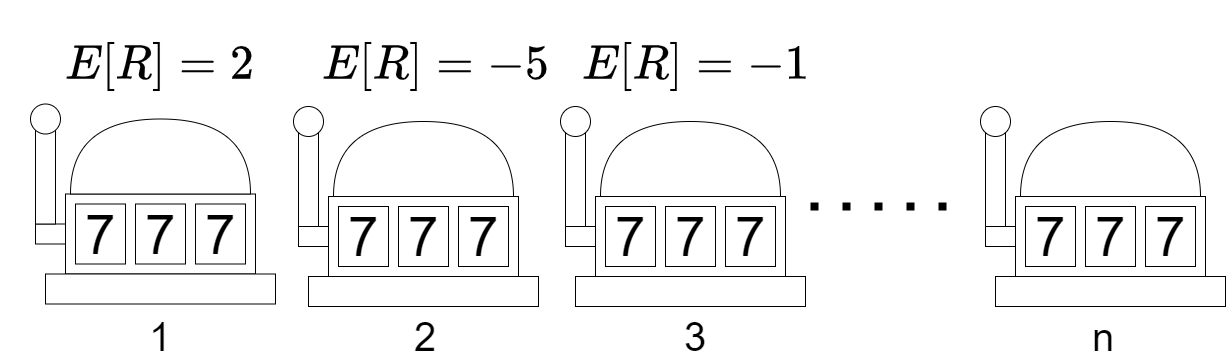
\includegraphics[width=1\textwidth]{losimoaparatai}
\caption{N lošimo aparatų, su skirtingais vidutiniais laimėjimais}
\label{losimoaparatai}
\end{figure}


Dažniausiai pateikiamas pavydzys, kuris iliustruoja šio mokslo principą bei padeda geriau suprasti šiuos kintamuosius, yra lošimo aparatu, pavaizduotų \ref{losimoaparatai} paveikslėlyje, laimėjimų optimizavimas. Šiame uždavinyje iš n aparatų agentas bando surasti lošimo aparatą, kuris suteikia dydžiausią įmanomą apdovanojimą. Kiekvienas aparatas duoda atsitiktinį laimėjimą iš  $\mathcal{N}(\mu=\mathcal{N}(0,2),\sigma=1)$ pasiskirstimo. Žaidimo sesija, dažniausiai vadiname episodas, nėra ribojima, agentas gali atlikti begalybe $t$ žingsnių, lošimo aparatų pasirinkimų. Pasirinkimą galima traktuoti kaip veiksmą $a$ ir gautą laimėjimą kaip $r$. Agentas bando vienos žaidimo sesijos metu įgyti dydžiausią sukauptą laimėjimą. Jis pritaiko viena iš populiariausiu skatinamojo mokslo metodu $\epsilon-greedy$. Šis metodas visados renkasi lošimo aparatą, kurio aproksimuotas tikėtinas laimėjimas, žymimas $Q(a)$, yra dydžiausias, kaip tai išreikšta \ref {eqn:argmaxA} formulėje.

\begin{equation}
\label{eqn:argmaxA}
\begin{gathered}
A_t = argmax_aQ_t(a)
\end{gathered}
\end{equation}

Tačiau su maža $\epsilon$ tikimybe, agentas pasirenka atsitiktinį lošimo aparatą. Taigi kiekviename $t$ žingsnyje agentas renkasi lošimo aparatą, jį aktyvuoja ir gauną naują apdovanojimą, kuri talpina į to aparato apdovanojimų sarašą. Šis procesas ypatingai svarbus, jis dominuoja visuose mokymosi modeliuose. Agentas stengiasi netik gauti dydžiausia įmanoma tikėtina laimėjimą, tačiau kartu tirinėja aplinką, ieško optimalesniu lošimo aparatu, nei surastas dabartinis geriausias. Šis procesas vadinasi apdovanojimų-tirinėjimo kompromisu. Lošimo aparato tikėtinas laimėjimas tėra to aparato gautų laimėjimų vidurkis, kaip tai matosi \ref{eqn:Q(a)} formulėje.

\begin{equation}
\label{eqn:Q(a)}
\begin{gathered}
Q_t(a) = \frac{\sum_{i=1}^{t-1}R_i*\mathbb{1}_{A_i=a}} {\sum_{i=1}^{t-1}\mathbb{1}_{A_i=a}}
\end{gathered}
\end{equation}

Kitaip tariant $Q_t(a)$ yra apdovanojimų suma, kuomet pasirinkome $a$ veiksmą (arba lošimo aparatą), atlikus $t$ žingsnių, padalinti iš kiek kartų buvo $a$ veiksmas (arba lošimo aparatas) pasirinktas. Kuomet $t$ artėja link begalybės, pagal didžiųjų skaičių dėsniu, $Q(a)$ priartėja prie tikrosios reikšmės. Visi naujausi modeliai yra paremti panašiu imties traukimo metodu - simuliuojame skirtingus veiksmus ir stebime gautus rezultatus. Nors pavyzdys atrodo primitivus, tačiau visi naujausi modeliai sprendžia tą pačią užduoti - kokį pasirinkti veiksmą $a$, kuris suteiktų dydžiausią apdovanojimą. 

Pagrindiniai skirtumai atsiranda dėl kompiuterio resursų optimizavimo. Viena iš problemu, su kuria iškarto susiduriame, yra duomenų kaupimas. Kiekvienam lošimo aparatui reikia kaupti jo gautus apdovanojimus. Didėjant problemai bei jos duomenų dimensijai, kompiuteriui kaupti duomenis tampa fiziškai nebeįmanoma, todėl yra sukurta daugybe esminių metodų šią problemą mažinti bei išvengti. Vienas iš metodų, kurio formą galima pastebėti TD formulėje, yra rekursyvus vidurkio apskaičiavimas, pateiktas \ref{eqn:Vidurkio} formulėje. Ši formule padeda išvengti apdovanojimų kaupimo, kaip tai matėme lošimo pavyzdyje.

\begin{equation}
\label{eqn:Vidurkio}
\begin{aligned}
Q_{n+1} &=\frac{1}{n} \sum_{i=1}^{n} R_{i} \\
&=\frac{1}{n}\left(R_{n}+\sum_{i=1}^{n-1} R_{i}\right) \\
&=\frac{1}{n}\left(R_{n}+(n-1) \frac{1}{n-1} \sum_{i=1}^{n-1} R_{i}\right) \\
&=\frac{1}{n}\left(R_{n}+(n-1) Q_{n}\right) \\
&=\frac{1}{n}\left(R_{n}+n Q_{n}-Q_{n}\right) \\
&=Q_{n}+\frac{1}{n}\left[R_{n}-Q_{n}\right]
\end{aligned}
\end{equation}

Lošimų pseudokodas, kuris palaipsniui apskaičiuoja skirtingų veiksmų imties vidurkius, pateiktas toliau:

\begin{algorithm}[H]
\label{LosimuAlgo}
\SetAlgorithmName{Algoritmas}{}
\SetAlgoLined

$Q(a) \leftarrow 0$\;
$N(a) \leftarrow 0$\;

 \For{$ \infty $}{
	$$ A \leftarrow \begin{cases}\arg \max _{a} Q(a) \text { su tikimybe } 1-\varepsilon \text { (lygiąsias reikšmes pasirenkame atsitiktinai) } \\
\text {atsitiktinis veiksmas } \text { su tikimybe} \varepsilon\end{cases}$$
	$R \leftarrow \text { LošimoAparatas }(A) $ \tcp*{Pasirenkame veiksma A ir gauname apdovanojimą R}
	$N(A) \leftarrow N(A)+1 $ \tcp*{Kiek kartų kiekvienas veiksmas buvo pasirinktas}
	$Q(A) \leftarrow Q(A)+\frac{1}{N(A)}[R-Q(A)]$\;
    }
\KwResult{ Gautos optimalios, tikrosios Q(a) reikšmės. Jas turint žinosime, kuris aparatas duoda dydžiausią laimėjimą}
 \caption{Lošimo aparato pseudo algoritmas}
\end{algorithm}


Paskutinė \ref{eqn:Vidurkio} formulės išraiška yra įpatingai svarbi, nes ji yra ištaka tiek TD, tiek Q-mokymosi, tiek bellmano formulėms, kurios yra skatinamojo mokslo pamatas. Apibendrinant formulę ją galima šitaip išreikšti:

\begin{equation}
\text{Naujas vidurkis = Senas vidurkis }+ \frac{1}{n} (\text{Nauja reikšmė - Senas vidurkis})
\end{equation}

Jei tęstume formules apibendrinimą išriškėtu bellmano funkcija, kuri yra viena svarbiausiu šiame moksle ir į kuria gilinsimes tolimesniuose skyriuose:

\begin{equation}
\label{TDLietuviskai}
\text{Naujas įvertis = Senas įvertis}+ \frac{1}{n} * (\textbf{Tikslas - Senas įvertis})
\end{equation}

Paryškinta dalis yra vadinama TD paklaida, ties kuria gilinsimes tolimesniuose skyriuose.

Kolkas nagrinėta problema pasižymi apdovanojimo skirstinio stacionarumu, jis nekinta. Tačiau nagrinėjant sudėtingas problemas netik mūsų apdovanojimų pasiskirstimas kinta, tačiau mum idomios tik paskutinės 10 -100 reikšmės bei aukštos dimensijos problemose mum neužtenka kompiuterio resursų išsaugoti $N(A)$ reikšmių, ką mes atliekame \ref{LosimuAlgo} pseudokode. Todėl įgyvendinamas dar vienas šios formulės optimizavimas

%
\subsubsection{Ne stacionarus pasiskirstymas}
%

Galima pastebėti daugybe problemų su \ref{eqn:Vidurkio} formule:

\begin{enumerate}
  \addtolength{\itemsep}{-0.5\baselineskip} 
  \item Toliau plėtojant duotą pavyzdį, galima įsivaizduoti situaciją, kurioje, kas tam tikrą laiko intervalą, kiekvieno aparato apdovanojimo funkcija pakinta ir įgyja nauja $\mathcal{N}(\mu=\mathcal{N}(0,2),\sigma=1)$ pasiskirstymą.
  \item Kuomet vieno lošimo aparato apdovanojimų $R$ imtis yra labai didelė, naujai gautos reikšmės turi labai mažai įtakos vidurkio pokyčiui dėl $\frac{1}{n}$ formulėje esančios išraiškos.
  \item Kiekviena $Q(a)$ reikšmė turi kaupti $N(A)$. Aukštosiose dimensijos neužtenka kompiuterio resursų išsaugoti šias reikšmes.
\end{enumerate}

Šios problemos sprendimas jau buvo pateiktas Adamo algoritmo įgyvendinime, mes toliau naudojame judančio vidurkio principus:

\begin{equation}
\label{judantisVidurkis}
\begin{aligned}
Q_{n+1} &=Q_{n}+\alpha\left[R_{n}-Q_{n}\right] \\
&=\alpha R_{n}+(1-\alpha) Q_{n} \\
&=\alpha R_{n}+(1-\alpha)\left[\alpha R_{n-1}+(1-\alpha) Q_{n-1}\right] \\
&=\alpha R_{n}+(1-\alpha) \alpha R_{n-1}+(1-\alpha)^{2} Q_{n-1} \\
&=\alpha R_{n}+(1-\alpha) \alpha R_{n-1}+(1-\alpha)^{2} \alpha R_{n-2}+\\
& \quad \ldots+(1-\alpha)^{n-1} \alpha R_{1}+(1-\alpha)^{n} Q_{1} \\
&=(1-\alpha)^{n} Q_{1}+\sum_{i=1}^{n} \alpha(1-\alpha)^{n-i} R_{i}
\end{aligned}
\end{equation}

Ši \ref{judantisVidurkis} formulė pakeičia $\frac{1}{n}$ į $\alpha \in [0,1]$. Dažniausia $\alpha$ reikšmė yra 0.9, su kuria apytiksliai apskaičiuojame paskutinių gautų 10-ties narių vidurkį.

\subsubsection{Markovo grandinės}

Dauguma mažos dimensijos skatinamojo mokslo problemų galima išreikšti markovo grandinių pavidalu. Toks išreiškimas padeda geriau suvokti keturias pagrindines skatinamojo mokslo savokas:

\begin{enumerate}
  \addtolength{\itemsep}{-0.5\baselineskip} 
  \item $s$ - esama būsena.
  \item $a$ - pasirinktas veiksmas.
  \item $r$ - esamosios būsenos pasirinkto veiksmo apdovanojimas.
  \item $s\sp{\prime}$ - nauja būsena, kuri gaunama atlikus $a$ veiksmą.
\end{enumerate}

Nors dažniausiai būsenos būna daugiau nei vienos dimensijos, pavyzdžiui būsenos vektorius susidedantis iš 2 reikšmių - pozicijos bei greičio, lengviausiai jas yra suprasti atvaizduojant vienos dimensijos markovo grandinių pavidalu, kaip tai matosi \ref{DulkiuSiurblys} paveikslėlyje.

\begin{figure}[h]
\centering
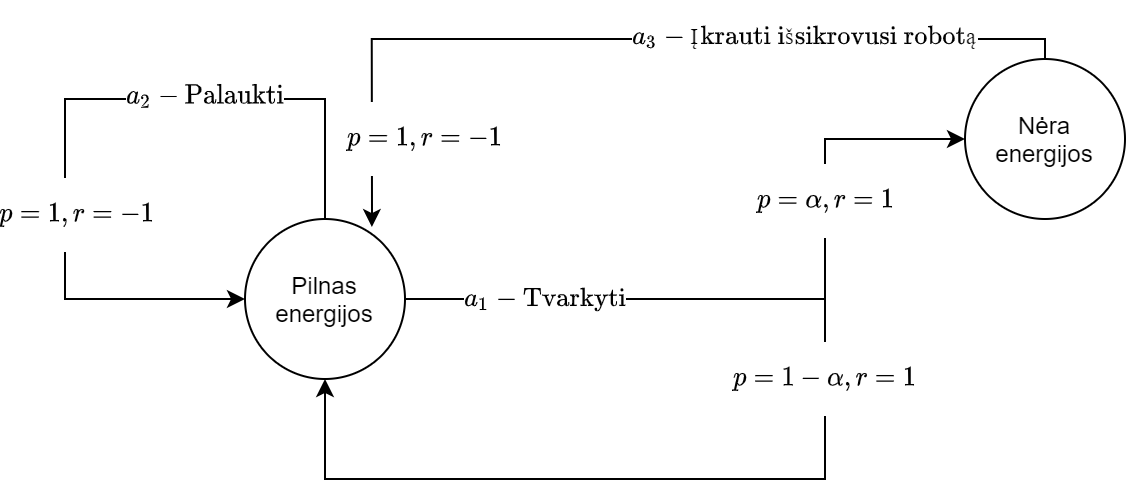
\includegraphics[width=1\textwidth]{DulkiuSiurblys}
\caption{Dulkio siurblio markovo grandinė}
\label{DulkiuSiurblys}
\end{figure}

Jei dulkio siurblio robotas yra būsenoje $s = \text{"Pilnas energijos"}$, jis gali pasirinkti $a_1$ arba $a_2$ veiksmus. Pasirinkęs $a_1$ veiksmą, robotas su $\alpha$ tikimybe gali patekti į būsena $s\sp{\prime} = \text{"Nėra energijos"}$ ir su tikimybe $1-\alpha$ į būseną $s\sp{\prime} = \text{"Pilnas energijos"}$. Už abu šiuos veiksmus veiksmus robotas yra apdovanojamas $r=1$. Šis procesas galioja ir kitoms būsenoms. 

Priklausomai nuo esančios būsenos, mes visa laika norime pasirinkti tokį veiksmą, kuris duoda dydžiausią tikėtiną apdovanojimą:

\begin{equation}
r(s, a) \doteq \mathbb{E}\left[R_{t} \mid S_{t-1}=s, A_{t-1}=a\right]=\sum_{r \in \mathcal{R}} r \sum_{s^{\prime} \in \mathcal{S}} p\left(s^{\prime}, r \mid s, a\right)
\end{equation}

Veiksmų pasirinkimas vadovaujantis dydžiausiu tikėtinu apdovanojimu bus nagrinėjamas sekančiame skyriuje.

Markovo grandinių išraiška taip pat yra svarbi ne tik dėl vizualinio aiškumo. Visos skatinamojo mokymo problemų formuluotės privalomai turi galėti išsireikšti markovo grandinių pavidalu. Šis reikalavimas yra būtinas dėl vienos iš pagrindinių markovo grandinės savybių - ateities įvykio tikimybė nepriklauso nuo prieš tai įvykusių įvykių:

\begin{equation}
P\left(X_{n+1}=x \mid X_{0}, X_{1}, X_{2}, \ldots, X_{n}\right)=P\left(X_{n+1}=x \mid X_{n}\right),
\end{equation}

kur $X$ yra prieš tai buvę įvykiai. Ši savybė leidžia apskaičiuoti tikėtiną apdovanojimą pasitelkiant tik turima busena, prieš tai buvusios būsenos neturi įtakos tikėtinam apdovanojimui.

Taigi \ref{DulkiuSiurblys} pavyzdys iliustruoja kaip skatinamajame moksle yra lengva apskaičiuoti naudingiausius veiksmus, kuomet turime sudaryta modelį. Tačiau retu atveju mes jį turime ir dažniausiai mum reikia imtis aplinkos tirinėjimo veiksmų, kurie sudaro modelio aproksimacijas. Taip pat mes ne tik norime apskaičiuoti geriausią sekančio veiksmo apdovanojimą, tačiau geriausią apdovanojimą ilgalaikėje perspektyvoje. Dažnai gyvenime mes pasirenkame mėgautis maloniais dalykais, kuriais vėliau mes gailimes. Būtent šią problemą kitas skyrius ir nagrinės - ilgalaikis apdovanojimas, o ne trumpalaikis.

\subsubsection{Apdovanojimai bei tikslai}

Adpovanojimų hipotezė: Kad visa tai, ką mes turime omenyje kalbėdami apie tikslus ir uždavinius, gali būti gerai suprantama kaip tikėtinos vertės maksimizavimas, kai gaunama ilgalaikė skalarinio signalo (vadinamo apdovanojimu) suma.

Šią sumą mes vieno epizodo metu stengemes maksimizuoti. Epizodas - būsenų, veiksmų, apdovanojimų seka, kuri užsibaige agentui pasiekus tikslą arba sustojimo sąlygą, kaip tai matome \ref{Episodas} paveikslėlyje. Agentas renkasi skirtingus veiksmus, įgauna naujas būsenas, kaupia epizodo apdovanojimą, kol galiausiai pasieke tikslą, pavaizduotų pilku kvadratu.

\begin{figure}[h]
\centering
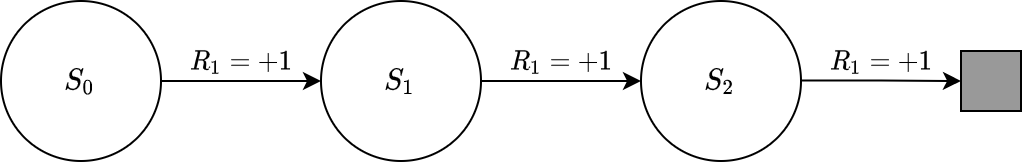
\includegraphics[width=0.8\textwidth]{Episodas}
\caption{Vienas agento epizodas}
\label{Episodas}
\end{figure}

Epizodo galutinis sukauptas apdovanojimas užrašomas tokiu pavidalu:

\begin{equation}
G_{t} \doteq R_{t+1}+R_{t+2}+R_{t+3}+\cdots+R_{T},
\end{equation}

kur $T$ yra paskutinis epizodo žingsnis. Tačiau jei agentas optimizuoja savo veiksmus aplinkoje, kurios pabaigą neįmanoma identifikuoti arba epizodas trunka nepaprastai daug žingsnių, mes naudojame apdovanojimų proporcionalius mažinimus:

\begin{equation}
G_{t} \doteq R_{t+1}+\gamma R_{t+2}+\gamma^{2} R_{t+3}+\cdots=\sum_{k=0}^{\infty} \gamma^{k} R_{t+k+1}
\end{equation}

kur $\gamma$ yra "nuolaidos" kintamasis, kurio dažniausia vertė yra 0.9. Ši vertė indikuoja, kad 11 žingsnio apdovanojimas bus proporcianalus $0.9^{11}$ savo vertės, kitaip tariant nuliui. Tačiau ši formulė kaip ir praeitos pasižymi panašiais trūkumais, kaip nuolatinis duomenų kaupimas. Tai galima išspręsti perrašius formulę į rekursinę formą:

\begin{equation}
\begin{aligned}
G_{t} & \doteq R_{t+1}+\gamma R_{t+2}+\gamma^{2} R_{t+3}+\gamma^{3} R_{t+4}+\cdots \\
&=R_{t+1}+\gamma\left(R_{t+2}+\gamma R_{t+3}+\gamma^{2} R_{t+4}+\cdots\right) \\
&=R_{t+1}+\gamma G_{t+1}
\end{aligned}
\end{equation}

Taip pat ši formulė padeda pasiekti balansą ties ilgalaikio apdovanojimo bei trumpalaikio apdovanojimo optimizavimo.

Vienas iš svarbiausių praktinių patarimų, padedančių pasiekti dydžiausią ilgalaikį apdovanojimą yra priskirti apdovanojimus už pasiektą tikslą, o ne skirti apdovanojimus už tai kaip mes norėtume, kad agentas pasiektų tikslą. Agentas mokymo procese turi pats atrasti optimaliausius veiksmus vedančius ties tiek tikslo pasiekimu, tiek dydžiausiu epizodo apdovanojimu. Kitame skyriuje bus apibrežiama, kaip būtent agentas optimizuoja savo elgesį, jo viena iš tikslo funkcijos konceptu, kurį gradientiniai metodai nuolatos optimizuoja.


\subsubsection{Vertės bei veiksmų taisyklių funkcijos}

Norint pasirinkti veiksmus, vedančius į būsenas, kurios suteikia dydžiausią įmanoma apdovanojimą, mes turime kiekvienai busenai priskirti tam tikrą matą. Todėl kiekviena būsena yra nusakoma pagal savo vertę. Ši vertė yra žymima $v_\pi(s)$ ir nusako pasirinktos $s$ būsenos tikėtiną apdovanojimą: 

\begin{equation}
v_{\pi}(s) \doteq \mathbb{E}_{\pi}\left[G_{t} \mid S_{t}=s\right]=\mathbb{E}_{\pi}\left[\sum_{k=0}^{\infty} \gamma^{k} R_{t+k+1} \mid S_{t}=s\right], \text { for all } s \in \mathcal{S}
\end{equation}

Žinant kiekvienos būsenos tikėtina apdovanojimą, mes visados galime rinktis tik tuos veiksmus, kurie veda į dydžiausią apdovanojimą, dydžiausią $v_\pi(s\sp{\prime})$. Šį pasirinkimą nusako veiksmų taisyklės. Tai yra tikimybių pasiskirstimas žymimas $\pi(a|s)$, nurodantis būsenos $s$ visų veiksmų pasirinkimu pasiskirstymą. Kitaip tariant su kokia tikimybe, mes pasirinktume veiksmą $a$ būnant būsenoje $s$, kaip tai matosi paveikslėlyje \ref{policy}.

\begin{figure}[h]
\centering
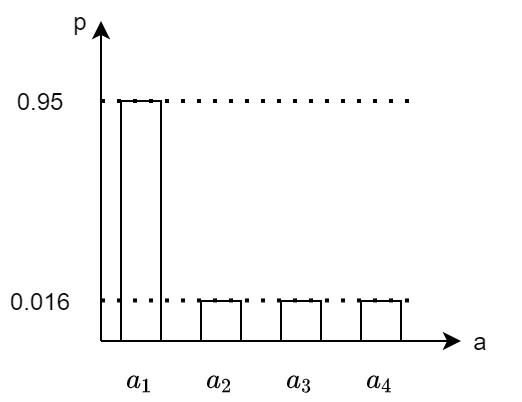
\includegraphics[width=0.6\textwidth]{policy}
\caption{Veiksmų taisyklių pasiskirstymas, kur $\epsilon=$5 }
\label{policy}
\end{figure}


Užrašymas $v_{\pi}(s)$ nurodo, kad ši būsenos vertė yra apskaičiuota naudojantis ${\pi}$ veiksmų taisyklėmis. Veiksmų taisyklės gali būti įvairios. Dažniausiai naudojame $\epsilon-greedy$ metodą, kaip tai matėme ties \ref{eqn:argmaxA} formule bei kurio pritaikymas markovo grandinėms yra pateiktas \ref{eqn:greedyPolicy} formulėje. Šio metodu mes visalaika priskiriame $1-\epsilon$ tikimybę veiksmui, kuris gražina dydžiausią apdovanojimą apskaičiuojama naudojantis $v_{\pi}(s)$ formule. 

\begin{equation}
\label{eqn:greedyPolicy}
\begin{aligned}
\pi^{\prime}(s) & \doteq \underset{a}{\arg \max } q_{\pi}(s, a) \\
&=\underset{a}{\operatorname{argmax}} \mathbb{E}\left[R_{t+1}+\gamma v_{\pi}\left(S_{t+1}\right) \mid S_{t}=s, A_{t}=a\right] \\
&=\underset{a}{\operatorname{argmax}} \sum_{s^{\prime}, r} p\left(s^{\prime}, r \mid s, a\right)\left[r+\gamma v_{\pi}\left(s^{\prime}\right)\right]
\end{aligned}
\end{equation}


Turint kiekvienos būsenos taisyklių pasiskirstymą, galima suskaičiuoti kiekvienos būsenos tikėtiną reikšmę, kaip tai matosi \ref {eqn:tiketinaReiksme} formulėje.

\begin{equation}
\label{eqn:tiketinaReiksme}
\begin{aligned}
v_{\pi}(s) & \doteq \mathbb{E}_{\pi}\left[G_{t} \mid S_{t}=s\right] \\
&=\mathbb{E}_{\pi}\left[R_{t+1}+\gamma G_{t+1} \mid S_{t}=s\right] \\
&=\sum_{a} \pi(a \mid s) \sum_{s^{\prime}} \sum_{r} p\left(s^{\prime}, r \mid s, a\right)\left[r+\gamma \mathbb{E}_{\pi}\left[G_{t+1} \mid S_{t+1}=s^{\prime}\right]\right] \\
&=\sum_{a} \pi(a \mid s) \sum_{s^{\prime}, r} p\left(s^{\prime}, r \mid s, a\right)\left[r+\gamma v_{\pi}\left(s^{\prime}\right)\right], \quad \text { kiekvienam } s \in \mathcal{S},
\end{aligned}
\end{equation}

Šios formulės paskutinė lygybė yra dar geriau žinoma kaip bellmano lygybė. Ji padeda rekursiškai apskaičiuoti $v_{\pi}(s)$ reikšmes bei išvengti apdovanojimų kaupimo kompiuterio atmintyje.

Tačiau praktikoje mes naudojame ne $v_{\pi}(s)$ - būsenos vertės matą, o $q_{\pi}(s, a)$ - veiksmo vertės matą esant būsenoj $s$:

\begin{equation}
q_{\pi}(s, a) \doteq \mathbb{E}_{\pi}\left[G_{t} \mid S_{t}=s, A_{t}=a\right]=\mathbb{E}_{\pi}\left[\sum_{k=0}^{\infty} \gamma^{k} R_{t+k+1} \mid S_{t}=s, A_{t}=a\right]
\end{equation}

Galime pastebėti, kad $v_{\pi}(s)$ yra tos būsenos $s$ visų veiksmų $q_{\pi}(s, a)$ proporcinga $\pi(a|s)$ sudėtis bei taip pat išsireiškia bellmano lygybe:

\begin{equation}
\begin{aligned}
& q_{\pi}(s, a)=E_{\pi}\left[G_{t} \mid S_{t}=s, A_{t}=a\right]=\\
&=\sum_{s^{\prime}} \sum_{r} p\left(s^{\prime}, r \mid s, a\right)\left[r+\gamma E_{\pi}\left[G_{t+1} \mid S_{t+1}=s^{\prime}\right]=\right.\\
=& \sum_{s^{\prime}} \sum_{r} p\left(s^{\prime}, r\mid s, a\right)\left[r \cdot \gamma \sum_{a^{\prime}} \pi\left(a^{\prime} \mid s^{\prime}\right) \cdot E_{\pi}\left[G_{t+1} \mid S_{t+1^{\prime}}=s^{\prime}, A_{t+1}=a^{\prime}\right]\right] \\
=& \sum_{s^{\prime}} \sum_{r} p\left(s^{\prime} r \mid s, a\right)\left[r+\gamma \sum_{a^{\prime}} \pi\left(a^{\prime} \mid s^{\prime}\right) \cdot q_{\pi}\left(s^{\prime}, a^{\prime}\right)\right],
\end{aligned}
\end{equation}

kur $v_{\pi}(s^{\prime}) = \gamma E_{\pi}\left[G_{t+1} \mid S_{t+1}=s^{\prime}\right]$.

$q_{\pi}(s, a)$ Formos dėka mum nereikia apskaičiuoti $s$ būsenos visų veiksmų apdovanojimus norint gauti $v_{\pi}(s)$. Užtenka rinktis tik tuos veiksmus, kurie yra jau apskaičiuoti bei optimaliausi.

Taigi turint būsenų verčių bei veiksmų taisyklių apskaičiavimo formules galime pradėti iteracini procesą, kurio tikslas yra optimizuoti šias reikšmes.

\subsubsection{Verčių bei veiksmų taisyklių iteravimas}

Optimizavimo metu, mes ieškome tokių būsenų verčių bei optimalių taisyklių, kurios gražintų dydžiausią epizodo apdovanojimą.
Yra daugybe būdų tai atlikti, kuriuos galima sugrupuoti į trys kategorijas:

\begin{enumerate}
  \addtolength{\itemsep}{-0.5\baselineskip} 
  \item Dinaminio programavimo metodas, kuomet modelis žinomas, mes kiekvienos iteracijos metu perskaičiuojame visas $v_{\pi}(s)$ reikšmes ir atnaujiname veiksmų taisykles. Šį procesą iteruojame, iki konvergacijos pasiekimo. Nenaudojamas metodas, nes labai retai tenkinama šio metodo privaloma salyga - modelio turėjimas. Modelį mes traktuojame kaip markovo grandinių modelį, su visų veiksmų perėjimo tikimybėmis.
  \item Monte Carlo metodai - imties metodais apskaičiuojame $q_{\pi}(s, a)$ reikšmes. Šis metodas taikomas kuomet neturime modelio ir reikia jį aproksimuoti. 
  \item Neuroninių tinklų aproksimacijos - metodai, kurie aproksimuoja $q_{\pi}(s, a)$ reikšmes. Jei monte carlo metodai apskaičiuodavo kiekvienos būsenos tikslias reikšmes, funkcijų aproksimacijos metodais mes jas apskaičiuojame tik apytiksliai.
\end{enumerate}

Visos šios kategorijos pasižymi bendru optimizavimo principu:

\begin{enumerate}
  \addtolength{\itemsep}{-0.5\baselineskip} 
  \item Įvertinimas - Perskaičiuojame $v_{\pi}(s)$ reikšmes naudojantis atnaujintomis veiksmų taisyklėmis.
  \item Tikslinimas - Turint naujas $v_{\pi}(s)$ reikšmes, perskaičiuojame optimalias veiksmų taisykles $\pi(a|s)$.
\end{enumerate}

\begin{figure}[h]
\centering
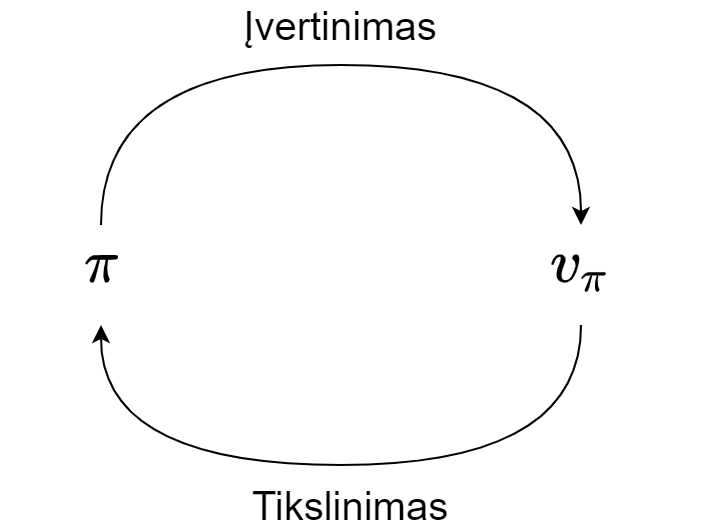
\includegraphics[width=0.5\textwidth]{policyIteration}
\caption{Viena optimizacijos iteracija }
\label{policyIteration}
\end{figure}

Šiuos žingsnius kartojame tol, kol pasiekiame $v_{\pi}(s)$ konvergaciją - naujos iteracijos nepakeičia $v_{\pi}(s)$ reikšmių. Tolimesniuose skyriuose trumpai apžvelgsiu šio proceso įgyvendinimą dinaminiuose bei monte karlo metoduose. Neuroninių tinklų aproksimacijos bus plėtojamos giliausiai, kadangi šiuo metu jie yra labiausiai paplite bei efektyviausi.

\subsubsection{Dinaminis programavimas}

Įvertinimo bei tikslinimo procesą, pateikta \label{policyIteration} paveikslėlyje, paprasčiausiai iliustruoja dinaminio programavimo metodas pateiktas \ref{DynamicProgrammingExample} pavyzdyje. Šiame pavyzdyje mūsų agentas atsiranda viename iš keturiolikos langeliu ir gali eiti į keturias puses, pateiktomis rodyklėmis. Agento tikslas patekti į žalius langelius. Kairėje paveikslėlio pusėje yra pateikti $v_{\pi}(s)$ įverčiai naudojantis \label{eqn:tiketinaReiksme} formule, o dešinėje perskaičiuojame optimalias veismų taisykles naudojantis \label{eqn:greedyPolicy} formule. Ypatingai svarbi optimizavimo seka:

\begin{enumerate}
  \addtolength{\itemsep}{-0.5\baselineskip} 
  \item Įvertinimas - Perskaičiuojame $v_{\pi}(s)$ reikšmes atnaujinamos naudojantis $t-1$ žingsnio taisyklėmis.
  \item Tikslinimas - Perskaičiavus $v_{\pi}(s)$ reikšmes, perskaičiuojame $t$ žingsnio optimalias veiksmų taisykles $\pi(a|s)$. Pavyzdyje naudojame godų veiksmo taisyklių įvertinima, kuris renkasi tik optimaliausius veiksmus.
\end{enumerate}

Vienas agento žingsnis, žymimas $t$, susideda iš šios įvertinimo bei tikslinimo sekos. Matome, kad užtenka vos tryjų žingsnių veiksmų taisyklėms tapti optimaliomis. Tačiau $v_{\pi}(s)$ reikšmėmių konvergacija užtrunka ilgesni laiką. Įvykus konvergacijai, agentui atsiradus ant bet kurio iš galimų baltų langelių, jis, vadovaudamasis veiksmų taisyklėmis, visados optimaliai suras kelią į žalius langelius. Taip pat labai svarbu pastebėti seniau aptarta $v_{\pi}(s)$ išsiskaidymą į $q_{\pi}(s, a)$ narių sumą. Šis išsiskaidymas intuityviai matosi pateiktame \ref{DynamicProgrammingExample} paveikslėlyje, kuomet kiekvieną rodyklę, galima traktuoti kaip $q_{\pi}(s, a)$ reikšmę. Šis išskaidymas yra svarbus neuroninių tinklų aproksimacijose, kaip tai bus aptarta tolimesniuose mokymosi modeliuose. Tačiau šis algoritmas yra tinkamas tik apskaičiuoti mažų dimensijų problemas bei iliustruoti intuityvius pavyzdžius. Augant tiek veiksmų, tiek būsenų erdvei šie skaičiavimai tampa neįmanomi. Ši problema plėtojama kitame skyriuje.


\begin{figure}[ht!]
\centering
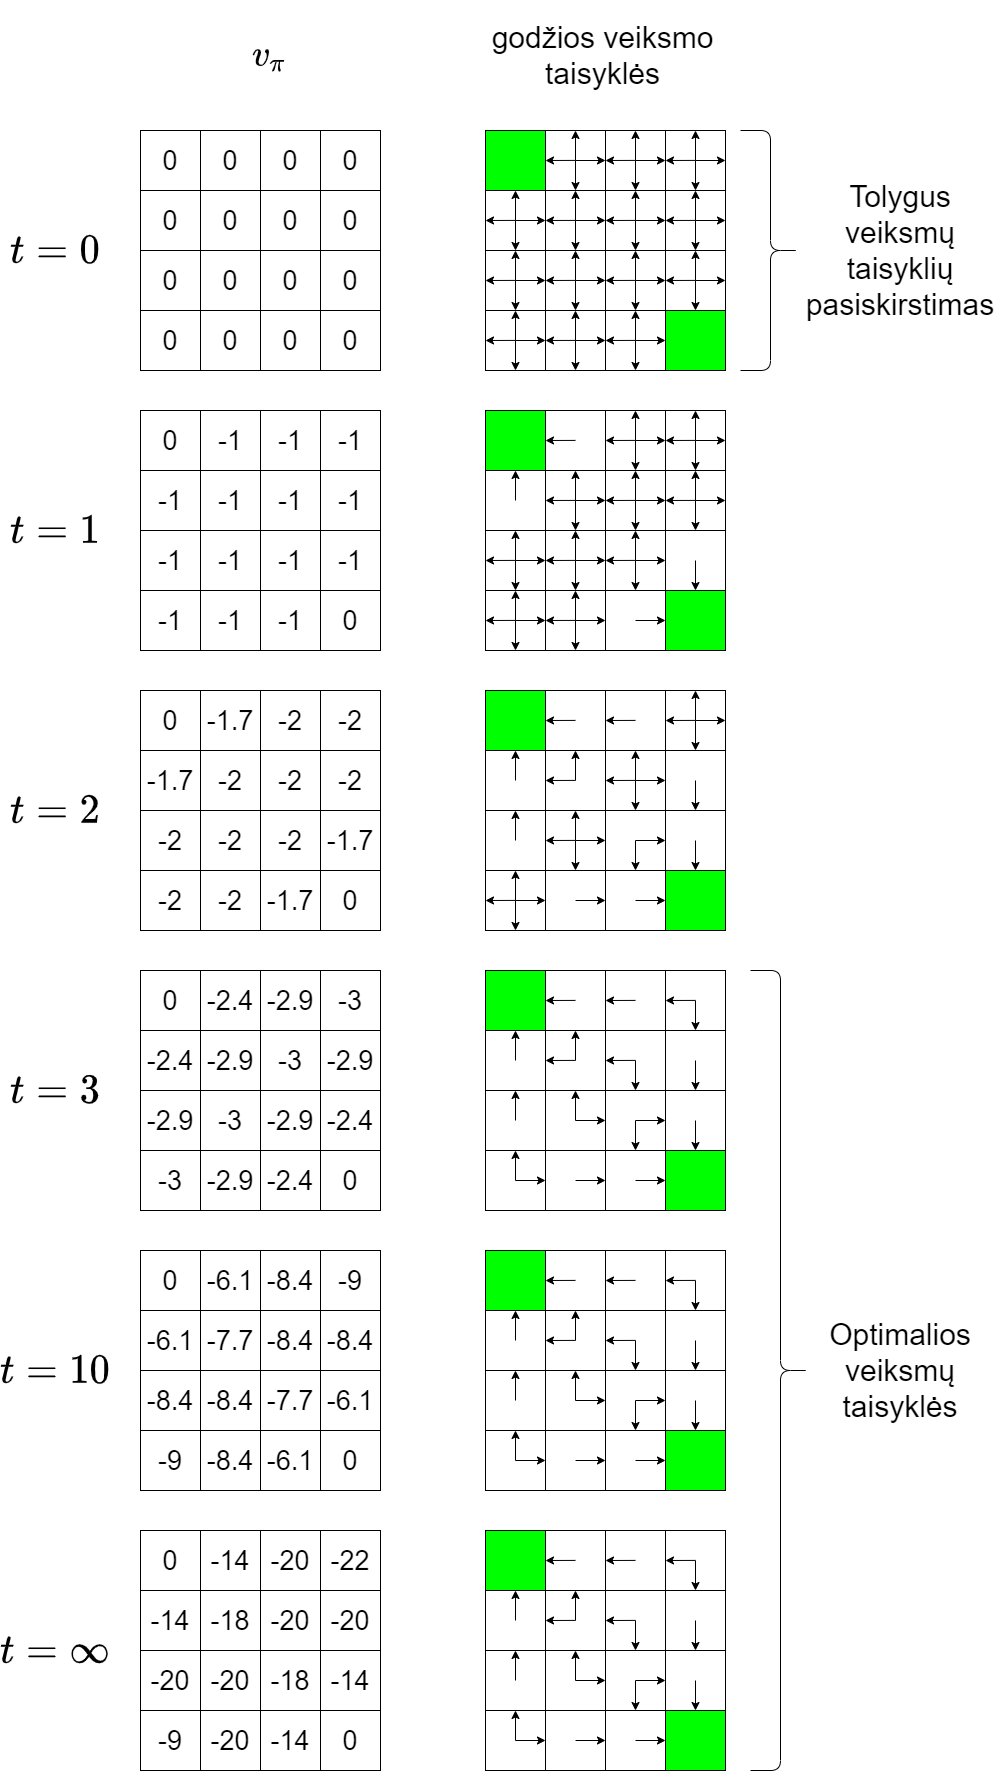
\includegraphics[width=0.8\textwidth]{DynamicProgrammingExample}
\caption{Dinaminio programavimo ve }
\label{DynamicProgrammingExample}
\end{figure}


\clearpage
\subsubsection{Monte Karlo metodai}

Nors specifinius Monte Carlo metodus šiame darbe nenagrinėsiu, tačiau pabrėšiu jų labai svarbų principą, kuriuo visi naujausi metodai remiasi. Monte Carlo metodais mes simuliuojame agento epizodus, gauname veiksmų trajektorijas (kaip tai matosi \ref{Episodas} paveikslėlyje) iš kurių susiskaičiuojame $q_{\pi}(s, a)$ reikšmes. Kiekvienos iteracijos metu kiekvienai būsenai $s$ bei jos specifiniui veiksmui $a$ mes išsaugome gautą apdovanojimą $G_t$. Iš šių išsaugotų reikšmių mes susiskaičiuojame vidurkį ir jį priskiriame $q_{\pi}(s, a)$ nariui. Tai atlikus mes perskaičiuojame veiksmų taisyklių reikšmes, kurios pasirenka naujus optimalius veiksmus. Po daugybes iteracijų, $q_{\pi}(s, a)$ konverguoja ties specifine, optimalia reikšme. Šio metodo veikimo principai pateikti \ref{alg:MC} pseudokode.

\begin{algorithm}[H]
 \label{alg:MC}
 \SetAlgorithmName{Algoritmas}{}
\SetAlgoLined
\DontPrintSemicolon
\textbf{Algoritmo parametrai:}\; 
$\varepsilon>0$\;
\textbf{Duomenų priskirimas:}\;

	$\pi \leftarrow$ atsitiktinė $\varepsilon$-greedy veiksmų taisyklių pasiskirstymas\;
	$Q(s, a) \in \mathbb{R}$ (atsitiktinis priskirimas), visiems $s \in \mathcal{S}, a \in \mathcal{A}(s)$\;
	Vertės $(s, a) \leftarrow$ tuščias sąrašas, visiems $s \in \mathcal{S}, a \in \mathcal{A}(s)$\;
	


 \For{$ \infty $}{
	Agentas sugeneruoja episodą sekant $\pi: S_{0}, A_{0}, R_{1}, \ldots, S_{T-1}, A_{T-1}, R_{T}$\;
	$G \leftarrow 0$\;
	 \For{$t=T-1, T-2, \ldots, 0$}{
		$G \leftarrow \gamma G+R_{t+1}$\;
		\uIf{ Jei $S_{t}, A_{t}$ būsena yra pirmas apsilankymas  $S_{0}, A_{0}, S_{1}, A_{1} \ldots, S_{t-1}, A_{t-1}$ sekoje}{
    		Išsaugoti $G$ į Vertės$\left(S_{t}, A_{t}\right)$ sąraša\;
			$Q\left(S_{t}, A_{t}\right) \leftarrow$ vidurkis $\left(\right.$ Vertės$\left.\left(S_{t}, A_{t}\right)\right)$\;
			$A^{*} \leftarrow \arg \max _{a} Q\left(S_{t}, a\right)$\;
  			}
			\For{visi $a \in \mathcal{A}\left(S_{t}\right)$}{
			$
			\pi\left(a \mid S_{t}\right) \leftarrow \begin{cases}1-\varepsilon+\varepsilon /\left|\mathcal{A}\left(S_{t}\right)\right| & \text { if 			} a=A^{*} \\ \varepsilon /\left|\mathcal{A}\left(S_{t}\right)\right| & \text { if } a \neq A^{*}\end{cases}\;
			$
			}
		}
    }
\KwResult{ Gautos optimalios $Q(s, a)$ bei $\pi(a|s)$ reikšmės.}
\caption{Taisyklių bei verčių aproksimavimas Monte Carlo pirmo apsilankymo metodu}
\end{algorithm}

\ref{alg:MC} Algoritmo problema, kaip ir prieš tai buvusių metododų, yra kiekvienos būsenos ir jo veiksmo saugojimas bei ilgas konvergavimas. Augant būsenų bei veiksmų dimensijoms, konvergavimas tampa neįgyvendinama užduotimi. Veiksmams bei dimensijoms užtenka būti trečioje dimensijoje ir jau nebeužtenka kompiuterio resursų apskaičiuoti optimalių reikšmių. Taip pat monte karlo metodai pasižymi duomenų kaupimo problema, kuomet neužtenka atminties juo saugoti. Duomenų kaupimą galima sumažinti pasitelkiant \ref{eqn:Vidurkio} bei \ref{judantisVidurkis} formulėmis, kaip tai atlieka pagrindinės šio mokslo formulės - TD ir Q-mokymasis.

\subsubsection{TD bei Q-mokymasis}

TD formulė sukombinuoja Monte Karlo bei dinaminio programavimo pagrindines idėjas į vieną paprastą \ref{TD} formulę. 

\begin{equation}
\label{TD}
\begin{aligned}
V\left(S_{t}\right) &\leftarrow V\left(S_{t}\right)+\alpha\left[G_{t}-V\left(S_{t}\right)\right] = \\
& = V\left(S_{t}\right)+\alpha\left[R_{t+1}+\gamma V\left(S_{t+1}\right)-V\left(S_{t}\right)\right]
\end{aligned}
\end{equation}

Šios formulės ištakas galima pastebėti tiek \ref{eqn:Vidurkio} bei \ref{judantisVidurkis} formulėse. Šias dvi formules sukombinavus, galime perrašyti \ref{eqn:tiketinaReiksme} formulę, kuri pasitelkia markovo grandinių modeliu, į \ref{TD} formulę, be markovo grandinių modelio. TD paklaida yra paklaida tarp $R_{t+1}+\gamma V\left(S_{t+1}\right)$ bei $V\left(S_{t}\right)$. Kuomet $V\left(S_{t}\right)$ konverguoja, TD paklaida tampa nulinė. Pasiekus nulinę TD paklaidą galima laikyti, kad modelis apsimokė. Vienas iš pagrindinių šio modelio skirtumu lyginant su \ref{alg:MC} algoritmu, yra greitesnė konvergacija. Šis metodas nelaukia epizodo galo, o atlieka $v_{\pi}(s)$ verčių atnaujinimą kiekvieno agento žingsnio metu. TD metodas yra pagrindas SARSA bei Q-mokymosi metodams, kurie atlieka atnaujinimus $q_{\pi}(s, a)$ vertėms. Šios dvi metodologijos skiriasi savo optimalumo atradimu, SARSA naudojasi šia TD atnaujinimo formule:

\begin{equation}
Q(S, A) \leftarrow Q(S, A)+\alpha\left[R+\gamma Q\left(S^{\prime}, A^{\prime}\right)-Q(S, A)\right].
\end{equation}

o Q-mokymasis šia:

\begin{equation}
\label{TD-Q}
Q(S, A) \leftarrow Q(S, A)+\alpha\left[R+\gamma \max _{a} Q\left(S^{\prime}, a\right)-Q(S, A)\right]
\end{equation}

Nors šios formulės yra vos ne identiškos, tačiau jos skiriasi skirtingomis optimaliomis veiksmų trajektorijomis. SARSA modelio atveju agentas stengesi elgtis saugiai, dažniau vengia būsenų, kurių vertė yra neigiama. Šis modelis tinkamas tokiems eksperimentams, kuriuos yra brangu simuliuoti ir norime sumažinti agento kritines klaidas besimokant, vedančias ties agento fiziniu sugedimu, praradimu. Šio atvejo pavyzdys galėtų būti roboto navigacija ties šlaitu. Kiekvienos simuliacijos metu agentui besimokant jis gali nukristi nuo šlaito ir sugadinti savo įranga. Todėl norint šias brangias klaidas sumažinti mes apmokome robota pasitelkiant SARSA metodu. Bet kadangi dydžiaja laiko dalį mokymasis vyksta simuliuotose aplinkose, mūsų agento kritinių klaidų kaina nėra faktorius. Svarbiausias tikslas mums tampa optimalios verčių suradimas, kuo Q-mokymasis ir pasižymi. Q-mokymasis \cite{QLearning} yra vienas iš populiariausių bei seniausių egzistuojančių metodu. Tačiau jis išpopuliarėjo visai neseniai, kuomet 2014 metais Google Deepmind komanda sugebėjo \ref{TD-Q} funkcija aproksimuoti pasitelkiant konvoliucinius neuroninius tinklus. Šiomis aproksimacijomis Deepmind komanda apmokė agentus įveikti Atari žaidimus taip pademonstruojant skatinamojo mokymosi bei neuroninių tinklų aproksimacijų potencialą. Visi dabartiniai modeliai pasitelkia neuroninių tinklų aproksimacijomis. Aproksimacijos padėjo išspręsti viena dydžiausių skatinamojo mokslo problemų - aukštų būsenų dimensijų neįmanoma konvergavimą. Dėl šios priežasties toliau bus aptariamas gilusisQ - vienas iš pirmųjų ir nors jau nebeefektyviu modeliu, sukėlusių skatinamojo mokslo atgimimą.

\subsubsection{Gilusis skatinamasis mokslas, gilusis-Q}

Visi naujausi, dabartiniai skatinamojo mokslo modeliai yra aproksimuojami neuroniniais tinklais. Neuroniniai tinklai padeda generalizuoti nepaprastai didžiules būsenų erdves, kaip tai pademonstravo Google Deepmind giliojo-Q konvoliucinis neuroninis tinklas, kurio įvestis buvo kompiuterio ekrano individualus pikseliai. 

Gilusis-Q metodas parametrizuoja $q_{\pi}(s, a, \theta)$ reikšmę. Jo $\theta$ parametrai tampa neuroninio tinklo $\theta$ parametrai, kurie yra gradientiniais metodais optimizuojami, su tikslu pasiekti tikrąsias optimalias $q_{\pi}(s, a)$ reikšmes. Gilusis-Q neuroninio tinklo išvestis yra aproksimuota $q_{\pi}(s, a)$ reikšmė, kuri yra pateikta Q-mokymosi \ref{TD-Q} formulėje šiuo $\left[R+\gamma \max _{a} Q\left(S^{\prime}, a\right)\right]$ pavidalu. Kaip matome, mus domina tik pateiktos funkcijos tikslo dalis, kaip tai išreikšta \ref{TDLietuviskai} formulėje. Šis tikslas yra traktuojamas, kaip naujausia $q_{\pi}(s, a)$ reikšmė. Dažnai norint tai pabrėžti Q-mokymosi formulė yra pertvarkoma į \ref{QTikslas} formulėje pateiktą bellmano pavidalą:

\begin{equation}
\label{QTikslas}
Q^{\text {naujas }}\left(s_{t}, a_{t}\right) \leftarrow(1-\alpha) \cdot \underbrace{Q\left(s_{t}, a_{t}\right)}_{\text{Sena reikšmė}}+\alpha \cdot\underbrace{(r_{t}+\gamma \cdot \max _{a} Q\left(s_{t+1}, a\right))}_{\text{Tikslas = nauja $q_{\pi}(s, a)$ reikšmė}}
\end{equation} 


Šis pavidalas yra nekaskitas, o daugybe kartu nagrinėta judančio vidurkio formulė, kur $\left[R+\gamma \max _{a} Q\left(S^{\prime}, a\right)\right]$ yra naujausia gauta $q_{\pi}(s, a)$ reikšmė.

Taigi neuroninis tinklas stengesi aproksimuoti tikslą, kuris geriau žinomas kaip $G_t$ arba naujausias aproksimuotas $q_{\pi}(s, a)$ narys. Tuo tarpu neuroninio tinklo įvestis yra būsenos vektorius $s$. Kadangi naudojamas neuroninis tinklas, vektoriaus $s$ dydis nėra svarbus, konvergacija išlieka sparti. 

Optimizavimo procesas susideda iš šių tryju dalių:

\begin{enumerate}
  \addtolength{\itemsep}{-0.5\baselineskip} 
  \item Sukuriama duomenų talpykla bei du neuroniniai tinklai - taikinys bei pagrindinis.
  \item Pasirenkame veiksmą vadovaujantis godžiuoju $\epsilon$ veiksmų taisyklių metodu
  \item Svorių atnaujinimas naudojantis bellmano taisykle, pateikta \ref{QTikslas}
\end{enumerate}

\paragraph{Patirčių talpyklos bei dviejų neuroninių tinklų sukurimas}

Agentas tyrinėdamas aplinką, kaupia duomenis patirčių talpykloje, dar kitaip vadinama buferiu. Ši patirčių talpykla yra agento praeities patirtys, kurios padeda optimizuoti neuroninius tinklus. Joje kaupiamos $(s,a,r,s^\prime)$ duomenų eilutės, kurios vos ne identiškos SARSA modelio duomenims. Panašumas ties tuo nesibaige, modelis taip pat kaupia duomenis tokiu pačiu principu kaip SARSA modelis, monte karlo budu simuliuojant žingsnius. Esant būsenoje $s$ pagrindinis neuroninis tinklas aproksimuoja $s$ būsenos visų $a$ veiksmų $q_{\pi}(s, a)$ vertes, kaip tai matyti \ref{QNeuroniniaiTinklai} paveikslėlyje ir pasirenka judėti ta trajektorija, kurios $q_{\pi}(s, a)$ vertė yra dydžiausia. 

\begin{figure}[h]
\centering
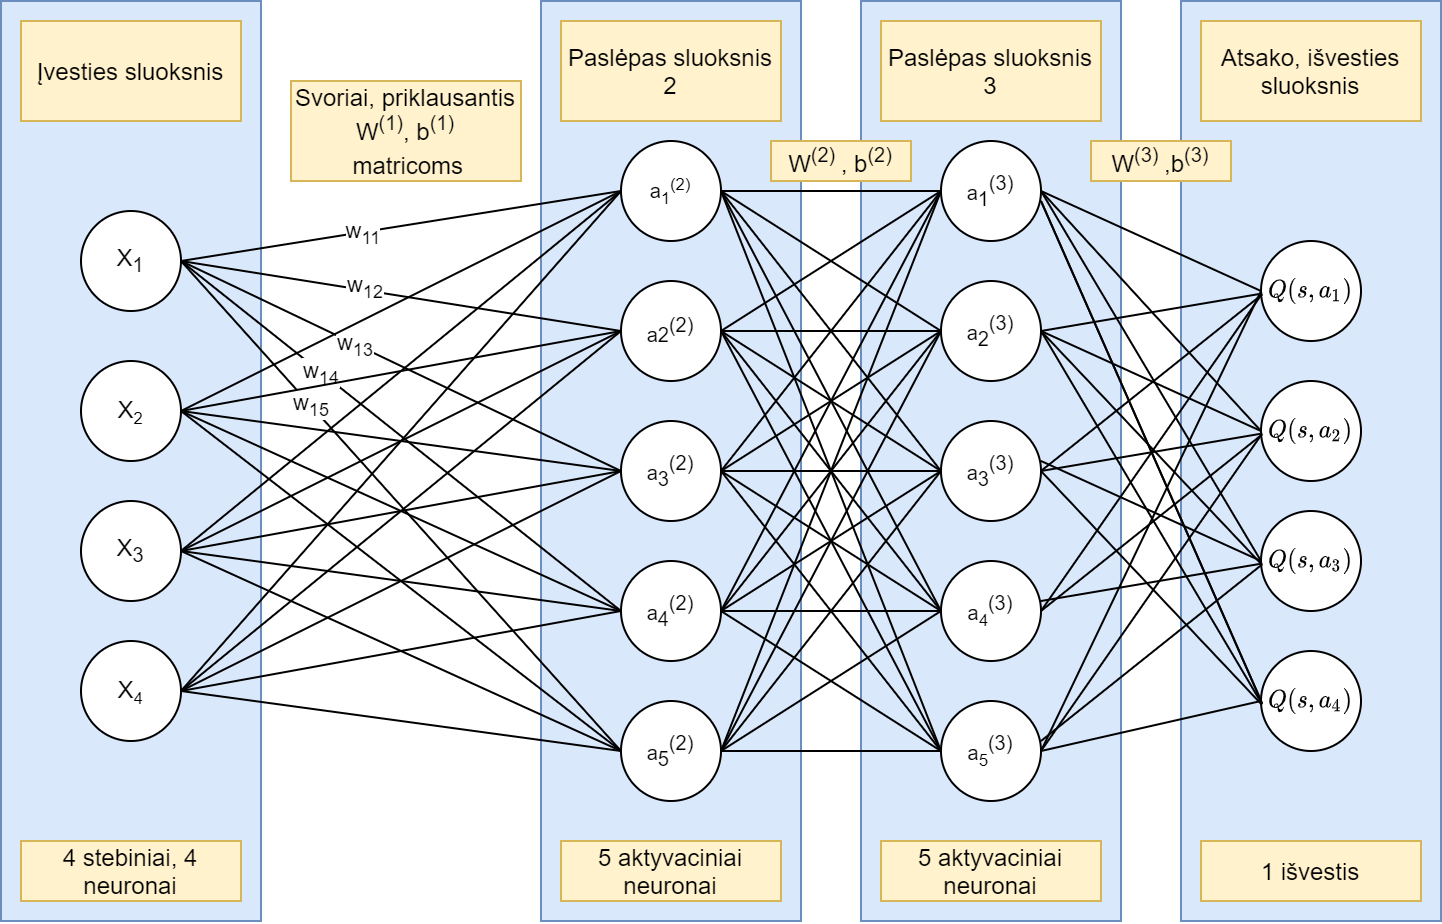
\includegraphics[width=1\textwidth]{Q Neuronu diagrama}
\caption{Giliojo Q neuroninio tinklo struktūra}
\label{QNeuroniniaiTinklai}
\end{figure}


Atlikus veiksmą mes apskaičiuojame gautą apdovanojimą $r$ bei naują buseną $s^\prime$, kurioje atsiradome atlikus veiksmą $a$. Tokiu budu turim vieną duomenų eilutę, kurią išsaugome į patirčių talpyklą. Sukaupus pakankamai daug duomenų galime juos pradėti naudoti neuroninio tinklo apmokymui. Apmokant mes pasitelkiame tik mažą dalį duomenų atsitiktinai ištrauktų iš talpyklos. Svarbu neuroninį tinklą apmokyti tik su duomenimis iš patirčių talpyklos, norint išvengti koreliacijos. Šią korelecijos tendencija lengva pastebėti intuityviai išanalizavus patyrčių talpyklos veikimo principus:

\begin{enumerate}
  \addtolength{\itemsep}{-0.5\baselineskip} 
  \item Atsitiktinės duomenų eilutės $(s,a,r,s^\prime)$ paimamos iš patirčių talpyklos. Dėl atsitiktinio ėmimo, dydžioji dalis patirčių - duomenų eilučių, yra iš skirtingų trajektorijų, epizodų.
  \item Su paimtais duomenimis apmokome modelį. Šio proceso metu, dėl atsitiktinio ėmimo, skirtingos būsenos įgyją naujas $q_{\pi}(s, a)$ aproksimacijas. 
\end{enumerate}

Tuo tarpu be patirčių talpyklos, mes apmokytume neuroninį tinklą kiekvieno žingsnio metu. Tačiau kadangi nauji agento žingsniai priklauso nuo senesnių, mūsų duomenis taptų priklausomi. Tai pažeidžia stochastinio gradientinio nuolydžio viena iš pagrindinių reikalavimų - imties duomenis turi būti nepriklausomi. Tai nutikus modelis pradėtų dažniau rinktis pasikartojančias trajektorijas, diverguotų į ne optimalias trajektorijas. Patirties talpykla taip pat turi dar viena papildoma svarbų bruožą - pakartotinas apmokymas su tais pačiais duomenimis. Kadangi duomenis yra išsaugojami talpykloje, mes turime ne mažą tikimybę apmokyti neuroninį tinklą su tuo pačiu dėmeniu ne vieną kartą. Šis bruožas naudingas apmokyti neuroninį tinklą su retai pasitaikančiomis reikšmėmis. Patirčių talpykla dažniausiai turi fiksuotą dydį. Talpykla yra naudojama visuose algoritmuose, kurie naudoja neuroninių tinklų aproksimacijas. 

Patirčių talpykla padeda apsimokyti pagrindiniam neuroniniui tinklui, kurio tikslo funkcija yra pateikta žemiau:

\begin{equation}
L(\theta)=\left[\left(\left(r+\gamma \max _{a t+1} Q\left(s_{t+1}, a_{t+1} ; \theta^{\text {taikinys }}\right)\right)-Q\left(s, a ; \theta^{\text {pagrindinis }}\right)\right)^{2}\right]
\end{equation}

Kaip matome $\theta$ parametrai atkeliauja iš taikinio bei pagrindinio neuroninio tinklo. Abu neuroniniai tinklai aproksimuoja $q_{\pi}(s, a)$. Tačiau taikinio neuroninio tinklo parametrai nėra apmokami, jie kas tam tikra agento žingsnių kieki yra periodiškai paimami iš pagrindinio neuroninio tinklo. Tuo tarpu pagrindinio neuroninio tinklo parametrai yra atnaujinami kas kiekviena žingsnį. Ši metodologija buvo pirma karta pritaikyta Google Deepmind komandos, kuriant Atari agentus \cite{GoogleDeepQLearning}. Jos tikslas yra sumažinti mokymosi divergacijas bei nestabilias $q_{\pi}(s, a)$ verčių svyravimus. Šios nepalankios savybės atsiranda iš neuroninių tinklų generalizacijos. Atnaujinus $q_{\pi}(s, a)$ reikšmes ir pakeitus $\theta$ parametrus, kartu pasikeičia kaimyninės $q_{\pi}(s^\prime, a)$ reikšmės, kitaip tariant mūsų taikinio reikšmės, jei naudotume viena neuroninį tinklą. Nuolat kintančios taikinio reikšmės veda prie nestabilaus konvergavimo, mūsų $q_{\pi}(s, a)$ reikšmės artėja link norimų $q_{\pi}(s, a)$ reikšmių, kurios dėl kiekvieno atnaujinimo kinta. Todėl yra sukuriamas antras neuroninis tinklas su fiksuotais parametrais, kurie stabilizuoja mokymosi procesą.




\paragraph{Veiksmų pasirinkimas}

\paragraph{Svorių atnaujinimas}







Q-mokymosi yra nebenaudojamas  nes įvyko vienas dydžiausių proveržių nes buvo įrodytas veiksmų taisyklių gradientas 


\subsubsection{Veiksmo taisyklių gradientas}

\begin{equation}
P(\tau \mid \theta)=\rho_{0}\left(s_{0}\right) \prod_{t=0}^{T} P\left(s_{t+1} \mid s_{t}, a_{t}\right) \pi_{\theta}\left(a_{t} \mid s_{t}\right)
\end{equation}


\begin{equation}
\nabla_{\theta} P(\tau \mid \theta)=P(\tau \mid \theta) \nabla_{\theta} \log P(\tau \mid \theta)
\end{equation}

\begin{equation}
\log P(\tau \mid \theta)=\log \rho_{0}\left(s_{0}\right)+\sum_{t=0}^{T}\left(\log P\left(s_{t+1} \mid s_{t}, a_{t}\right)+\log \pi_{\theta}\left(a_{t} \mid s_{t}\right)\right)
\end{equation}

\begin{equation}
\begin{aligned}
\nabla_{\theta} \log P(\tau \mid \theta) &=\nabla_{\theta} \log _{0}\left(s_{0}\right)+\sum_{t=0}^{T}\left(\underline{\nabla_{\theta} \log P\left(s_{t+1} \mid s_{t}, a_{t}\right)}+\nabla_{\theta} \log \pi_{\theta}\left(a_{t} \mid s_{t}\right)\right) \\
&=\sum_{t=0}^{T} \nabla_{\theta} \log \pi_{\theta}\left(a_{t} \mid s_{t}\right)
\end{aligned}
\end{equation}

\subsubsection{TODO}

-qmokymasis, bufferis
-policy gradient
-aktorius kritikas
-DDPG
-TD3

%-pakeist * i \cdot
%
\subsubsection{Pirmo skyriaus skyrelio poskyris}
%
Nunc eleifend consequat lorem. Sed lacinia nulla vitae enim. Pellentesque 
tincidunt purus vel magna. Integer non enim. Praesent euismod nunc eu purus. 
Donec bibendum quam in tellus. Nullam cursus pulvinar lectus. Donec et mi. 
Nam vulputate metus eu enim. Vestibulum pellentesque felis eu massa.
%
\paragraph{Pirmo skyriaus skyrelio poskyrio paragrafas.} 
%

Sed lacinia nulla vitae enim. Pellentesque tincidunt purus vel magna. Integer 
non enim. Praesent euismod nunc eu purus. Donec bibendum quam in tellus. 
Nullam cursus pulvinar lectus. Donec et mi. Nam vulputate metus eu enim. 
Vestibulum pellentesque felis eu massa.
%
%
\subsection{Skatinamasis mokslas}
hehe
%
%






\newpage
% ------------------------------------------------------------------- IŠVADOS --
\section*{Išvados}
\phantomsection
\addcontentsline{toc}{section}{Išvados}
%
Nulla malesuada porttitor diam. Donec felis erat, congue non, volutpat at, 
tincidunt tristique, libero. Vivamus viverra fermentum felis. Donec nonummy 
pellentesque ante. Phasellus adipiscing semper elit. Proin fermentum massa ac 
quam. Sed diam turpis, molestie vitae, placerat a, molestie nec, leo. 
Maecenas lacinia. Nam ipsum ligula, eleifend at, accumsan nec, suscipit a, 
ipsum. Morbi blandit ligula feugiat magna. Nunc eleifend consequat lorem. Sed 
lacinia nulla vitae enim. 



Lentelė \ref{lentele} is an example of a referenced \LaTeX{} element.

\begin{table}[h!]
\centering
\begin{tabular}{||c c c c||} 
 \hline
 Col1 & Col2 & Col2 & Col3 \\ [0.5ex] 
 \hline\hline
 1 & 6 & 87837 & 787 \\ 
 2 & 7 & 78 & 5415 \\
 3 & 545 & 778 & 7507 \\
 4 & 545 & 18744 & 7560 \\
 5 & 88 & 788 & 6344 \\ [1ex] 
 \hline
\end{tabular}
\caption{Table to test captions and labels.}
\label{lentele}
\end{table}


\newpage
% ---------------------------------------------------------------- LITERATŪRA --
\phantomsection
\addcontentsline{toc}{section}{Literatūra}

% Bibliografija nėra įprastas skyrius, todėl į LaTeX dokumento turinį neįtraukiama. 
% Norint, kad bibliografija būtų įtraukiama į turinį, tenka sukurti fiktyvų skyrių 
% ir nurodyti, kaip jis bus atvaizduojamas turinyje.

\begin{thebibliography}{99}

\bibitem{TDSutton} 
Sutton, R. \& Barto, A. 1987, ‘A Temporal-Difference Model of Classical Conditioning’, in Proceedings of the Ninth Annual Conference of the Cognitive Science Society, Seattle, WA, pp. 355–78.\href{http://incompleteideas.net/papers/sutton-barto-TD-87.pdf}{PDF}.

\bibitem{QLearning}
Watkins, C.J.C.H. (1989). Learning from Delayed Rewards (PDF) (Ph.D. thesis). University of Cambridge. EThOS uk.bl.ethos.330022/ \href{https://www.cs.rhul.ac.uk/~chrisw/new_thesis.pdf}{PDF}

\bibitem{DeepQLearning}
 "Methods and Apparatus for Reinforcement Learning, US Patent \#20150100530A1" (PDF). US Patent Office. 9 April 2015. Retrieved 28 July 2018. \href{https://patentimages.storage.googleapis.com/71/91/4a/c5cf4ffa56f705/US20150100530A1.pdf}{PDF}

\bibitem{GoogleDeepQLearning}
Human-level control through deep reinforcement learning \href{https://storage.googleapis.com/deepmind-media/dqn/DQNNaturePaper.pdf}{PDF}


\end{thebibliography}
%
%
\newpage
% ------------------------------------------------------------------- PRIEDAI --
\appendix
\section{Priedai}


\end{document}
% ------------------------------------------------------------------------------
%  DOKUMENTO PABAIGA
% ------------------------------------------------------------------------------
